% !Mode:: "TeX:UTF-8"

\def\usewhat{pdflatex}                               % 定义编译方式 dvipdfmx 或者 pdflatex,默认为 dvipdfmx
                                                     % 方式编译,如果需要修改,只需改变花括号中的内容即可。
\documentclass[12pt,openany,oneside,ctexartutf8]{book}
                                                     % 本科生毕业论文通常采用单页排版
% !Mode:: "TeX:UTF-8"
%  Authors: 张井   Jing Zhang: prayever@gmail.com     天津大学2010级管理与经济学部信息管理与信息系统专业硕士生
%           余蓝涛 Lantao Yu: lantaoyu1991@gmail.com  天津大学2008级精密仪器与光电子工程学院测控技术与仪器专业本科生

%%%%%%%%%% Package %%%%%%%%%%%%
\usepackage{graphicx}                       % 支持插图处理
% \usepackage[a4paper,text={146.4true mm,239.2 true mm},top= 25.4true mm, bottom= 25.4true mm, left=31.7 true mm,head=6true mm,headsep=6.5true mm,foot=16.5true mm]{geometry}
\usepackage[a4paper,top=25.4mm, bottom=25.4mm, left=31.7mm, right=31.7mm, head=6true mm,headsep=6.5true mm,foot=17.5mm]{geometry}
                                            % 支持版面尺寸设置
\usepackage[squaren]{SIunits}               % 支持国际标准单位

\usepackage{titlesec}                       % 控制标题的宏包
\usepackage{titletoc}                       % 控制目录的宏包
\usepackage{fancyhdr}                       % fancyhdr宏包 支持页眉和页脚的相关定义
\usepackage[UTF8, fontset=windows]{ctex}                    % 支持中文显示
\usepackage{CJKpunct}
\usepackage{color}                          % 支持彩色
\usepackage{amsmath}                        % AMSLaTeX宏包 用来排出更加漂亮的公式
\usepackage{amssymb}                        % 数学符号生成命令
\usepackage[below]{placeins}    %允许上一个section的浮动图形出现在下一个section的开始部分,还提供\FloatBarrier命令,使所有未处理的浮动图形立即被处理
\usepackage{multirow}                       % 使用Multirow宏包,使得表格可以合并多个row格
\usepackage{booktabs}                       % 表格,横的粗线;\specialrule{1pt}{0pt}{0pt}
\usepackage{longtable}                      % 支持跨页的表格。
\usepackage{tabularx}                       % 自动设置表格的列宽
\usepackage{subfigure}                      % 支持子图 %centerlast 设置最后一行是否居中
\usepackage[subfigure]{ccaption}            % 支持子图的中文标题
\usepackage[sort&compress,numbers]{natbib}  % 支持引用缩写的宏包
\usepackage{enumitem}                       % 使用enumitem宏包,改变列表项的格式
\usepackage{calc}                           % 长度可以用+ - * / 进行计算
\usepackage{txfonts}                        % 字体宏包
\usepackage{bm}                             % 处理数学公式中的黑斜体的宏包
\usepackage[amsmath,thmmarks,hyperref]{ntheorem}  % 定理类环境宏包,其中 amsmath 选项用来兼容 AMS LaTeX 的宏包
\usepackage{CJKnumb}                        % 提供将阿拉伯数字转换成中文数字的命令
\usepackage{indentfirst}                    % 首行缩进宏包
\usepackage{CJKutf8}                        % 用在UTF8编码环境下,它可以自动调用CJK,同时针对UTF8编码作了设置

% \usepackage{fancybox} 

%\usepackage{hypbmsec}                      % 用来控制书签中标题显示内容
\newcommand{\tabincell}[2]{\begin{tabular}{@{}#1@{}}#2\end{tabular}}
\usepackage{xcolor}
%支持代码环境
\usepackage{listings}
\lstset{numbers=left,
language=[ANSI]{C},
numberstyle=\tiny,
extendedchars=false,
showstringspaces=false,
breakatwhitespace=false,
breaklines=true,
captionpos=b,
keywordstyle=\color{blue!70},
commentstyle=\color{red!50!green!50!blue!50},
frame=shadowbox,
rulesepcolor=\color{red!20!green!20!blue!20}
}
%支持算法环境
\usepackage[boxed,ruled,lined]{algorithm2e}
\usepackage{algorithmic}

\usepackage{array}
\newcommand{\PreserveBackslash}[1]{\let\temp=\\#1\let\\=\temp}
\newcolumntype{C}[1]{>{\PreserveBackslash\centering}p{#1}}
\newcolumntype{R}[1]{>{\PreserveBackslash\raggedleft}p{#1}}
\newcolumntype{L}[1]{>{\PreserveBackslash\raggedright}p{#1}}

% 生成有书签的 pdf 及其生成方式。通常可以在 tjumain.tex 文件的第一行选择 pdflatex 或者是 dvipdfmx 编译手段。如果选择前者,则使用 pdflatex + pdflatex 编译; 如果选择后者,在编译的时候选择 latex + bibtex + latex + latex 编译。出现混淆的时候,系统会报错。
% 如果您的pdf制作中文书签有乱码使用如下命令,就可以解决了
\def\atemp{pdflatex}\ifx\atemp\usewhat
\usepackage{cmap}                           % pdflatex 编译时,可以生成可复制、粘贴的中文 PDF 文档, 缺点是在Windows上显示时效果不大好,字体发虚
\usepackage{hyperref}
\hypersetup{
    unicode,
    pdfborder={0 0 0},
}
\fi
% \usepackage[pdftex,unicode,
%             CJKbookmarks=true,
%             bookmarksnumbered=true,
%             bookmarksopen=true,
%             colorlinks=false,
%             pdfborder={0 0 0},
%             citecolor=blue,
%             linkcolor=red,
%             anchorcolor=green,
%             urlcolor=blue,
%             breaklinks=true
%             ]{hyperref}

                                % 定义本文所使用宏包
\graphicspath{{figures/}}                            % 定义所有的 .eps 文件在 figures 子目录下
\begin{document}                                     % 开始全文
\begin{CJK*}{UTF8}{song}                             % 开始中文字体使用
	% !Mode:: "TeX:UTF-8"
%  Authors: 张井   Jing Zhang: prayever@gmail.com     天津大学2010级管理与经济学部信息管理与信息系统专业硕士生
%           余蓝涛 Lantao Yu: lantaoyu1991@gmail.com  天津大学2008级精密仪器与光电子工程学院测控技术与仪器专业本科生

% 2018/5/23修正
%           李幼萌 Youmeng Li: liyoumeng@tju.edu.cn   天津大学软件学院软件工程系

%%%%%%%%%%%%%%%%% Fonts Definition and Basics %%%%%%%%%%%%%%%%%
\newcommand{\song}{\CJKfamily{song}}    % 宋体
\newcommand{\fs}{\CJKfamily{fs}}        % 仿宋体
\newcommand{\kai}{\CJKfamily{kai}}      % 楷体
\newcommand{\hei}{\CJKfamily{hei}}      % 黑体
\newcommand{\li}{\CJKfamily{li}}        % 隶书
\newcommand{\yihao}{\fontsize{26pt}{26pt}\selectfont}       % 一号, 单倍行距
\newcommand{\xiaoyi}{\fontsize{24pt}{24pt}\selectfont}      % 小一, 单倍行距
\newcommand{\erhao}{\fontsize{22pt}{1.25\baselineskip}\selectfont}       % 二号, 1.25倍行距
\newcommand{\xiaoer}{\fontsize{18pt}{18pt}\selectfont}      % 小二, 单倍行距
\newcommand{\sanhao}{\fontsize{16pt}{16pt}\selectfont}      % 三号, 单倍行距
\newcommand{\xiaosan}{\fontsize{15pt}{15pt}\selectfont}     % 小三, 单倍行距
\newcommand{\sihao}{\fontsize{14pt}{14pt}\selectfont}       % 四号, 单倍行距
\newcommand{\xiaosi}{\fontsize{12pt}{12pt}\selectfont}      % 小四, 单倍行距
\newcommand{\wuhao}{\fontsize{10.5pt}{10.5pt}\selectfont}   % 五号, 单倍行距
\newcommand{\xiaowu}{\fontsize{9pt}{9pt}\selectfont}        % 小五, 单倍行距

\CJKtilde  % 重新定义了波浪符~的意义
\newcommand\prechaptername{第}
\newcommand\postchaptername{章}

\punctstyle{hangmobanjiao}             % 调整中文字符的表示,行内占一个字符宽度,行尾占半个字符宽度

% 调整罗列环境的布局
\setitemize{leftmargin=3em,itemsep=0em,partopsep=0em,parsep=0em,topsep=-0em}
\setenumerate{leftmargin=3em,itemsep=0em,partopsep=0em,parsep=0em,topsep=0em}

% 避免宏包 hyperref 和 arydshln 不兼容带来的目录链接失效的问题。
\def\temp{\relax}
\let\temp\addcontentsline
\gdef\addcontentsline{\phantomsection\temp}

% 自定义项目列表标签及格式 \begin{publist} 列表项 \end{publist}
\newcounter{pubctr} %自定义新计数器
\newenvironment{publist}{%%%%%定义新环境
\begin{list}{[\arabic{pubctr}]} %%标签格式
    {
     \usecounter{pubctr}
     \setlength{\leftmargin}{2.5em}   % 左边界 \leftmargin =\itemindent + \labelwidth + \labelsep
     \setlength{\itemindent}{0em}     % 标号缩进量
     \setlength{\labelsep}{1em}       % 标号和列表项之间的距离,默认0.5em
     \setlength{\rightmargin}{0em}    % 右边界
     \setlength{\topsep}{0ex}         % 列表到上下文的垂直距离
     \setlength{\parsep}{0ex}         % 段落间距
     \setlength{\itemsep}{0ex}        % 标签间距
     \setlength{\listparindent}{0pt}  % 段落缩进量
    }}
{\end{list}}

\makeatletter
\renewcommand\normalsize{
  \@setfontsize\normalsize{12pt}{12pt} % 小四对应 12 pt
  \setlength\abovedisplayskip{4pt}
  \setlength\abovedisplayshortskip{4pt}
  \setlength\belowdisplayskip{\abovedisplayskip}
  \setlength\belowdisplayshortskip{\abovedisplayshortskip}
  \let\@listi\@listI}
\def\defaultfont{\renewcommand{\baselinestretch}{1.63}\normalsize\selectfont} % 设置行距

\renewcommand{\CJKglue}{\hskip -0.1 pt plus 0.08\baselineskip} % 控制字间距,使每行 34 个汉字
\makeatother

%%%%%%%%%%%%% Contents %%%%%%%%%%%%%%%%%
\renewcommand{\contentsname}{目\qquad 录}
\setcounter{tocdepth}{1} % 控制目录深度
\titlecontents{chapter}[2em]{\vspace{.5\baselineskip}\xiaosan\song}
             {\prechaptername\CJKnumber{\thecontentslabel}\postchaptername\qquad}{}
             {\hspace{.5em}\titlerule*[10pt]{$\cdot$}\sihao\contentspage}
\titlecontents{section}[4.2em]{\vspace{.25\baselineskip}\sihao\song}
             {\thecontentslabel\quad}{}
             {\hspace{.5em}\titlerule*[10pt]{$\cdot$}\sihao\contentspage}
% \titlecontents{subsection}[4em]{\vspace{.25\baselineskip}\xiaosi\song}
%              {\thecontentslabel\quad}{}
%              {\hspace{.5em}\titlerule*[10pt]{$\cdot$}\sihao\contentspage}

%%%%%%%%%% Chapter and Section %%%%%%%%%%%%%
\setcounter{secnumdepth}{4}
\setlength{\parindent}{2em}

\renewcommand{\chaptername}{\prechaptername\CJKnumber{\thechapter}\postchaptername}
\titleformat{\chapter}{\centering}{\xiaosan\song}{\chaptername}{} %{2em}
\titlespacing{\chapter}{0pt}{0.1\baselineskip}{0.8\baselineskip}

\titleformat{\section}{\sihao\hei}{\thesection}{1em}{}
\titlespacing{\section}{0pt}{0.15\baselineskip}{0.25\baselineskip}

\titleformat{\subsection}{\sihao\hei}{\thesubsection}{1em}{}
\titlespacing{\subsection}{0pt}{0.1\baselineskip}{0.3\baselineskip}

\titleformat{\subsubsection}{\sihao\hei}{\thesubsubsection}{1em}{}
\titlespacing{\subsubsection}{0pt}{0.05\baselineskip}{0.1\baselineskip}

%%%%%%%%%% Table, Figure and Equation %%%%%%%%%%%%%%%%%
\renewcommand{\tablename}{表}                                     % 插表题头
\renewcommand{\figurename}{图}                                    % 插图题头
\renewcommand{\thefigure}{\arabic{chapter}-\arabic{figure}}       % 使图编号为 7-1 的格式 %\protect{~}
\renewcommand{\thesubfigure}{\alph{subfigure})}                   % 使子图编号为 a) 的格式
\renewcommand{\thesubtable}{(\alph{subtable})}                    % 使子表编号为 (a) 的格式
\renewcommand{\thetable}{\arabic{chapter}-\arabic{table}}         % 使表编号为 7-1 的格式
\renewcommand{\theequation}{\arabic{chapter}-\arabic{equation}}   % 使公式编号为 7-1 的格式

%%%%%% 定制浮动图形和表格标题样式 %%%%%%
\makeatletter
\long\def\@makecaption#1#2{
   \vskip\abovecaptionskip
   \sbox\@tempboxa{\centering\wuhao\song{#1\qquad #2} }
   \ifdim \wd\@tempboxa >\hsize
     \centering\wuhao\song{#1\qquad #2} \par
   \else
     \global \@minipagefalse
     \hb@xt@\hsize{\hfil\box\@tempboxa\hfil}
   \fi
   \vskip\belowcaptionskip}
\makeatother
\captiondelim{~~~~} %用来控制longtable表头分隔符

%%%%%%%%%% Theorem Environment %%%%%%%%%%%%%%%%%
\theoremstyle{plain}
\theorembodyfont{\song\rmfamily}
\theoremheaderfont{\hei\rmfamily}
\newtheorem{theorem}{定理~}[chapter]
\newtheorem{lemma}{引理~}[chapter]
\newtheorem{axiom}{公理~}[chapter]
\newtheorem{proposition}{命题~}[chapter]
\newtheorem{prop}{性质~}[chapter]
\newtheorem{corollary}{推论~}[chapter]
\newtheorem{definition}{定义~}[chapter]
\newtheorem{conjecture}{猜想~}[chapter]
\newtheorem{example}{例~}[chapter]
\newtheorem{remark}{注~}[chapter]
%\newtheorem{algorithm}{算法~}[chapter]
\newenvironment{proof}{\noindent{\hei 证明:}}{\hfill $ \square $ \vskip 4mm}
\theoremsymbol{$\square$}

%%%%%%%%%% Page: number, header and footer  %%%%%%%%%%%%%%%%%

%\frontmatter 或 \pagenumbering{roman}
%\mainmatter 或 \pagenumbering{arabic}
\makeatletter
\renewcommand\frontmatter{\clearpage
  \@mainmatterfalse
  }
\makeatother

%%%%%%%%%%%% References %%%%%%%%%%%%%%%%%
\renewcommand{\bibname}{参考文献}
% 重定义参考文献样式,来自thu
\makeatletter
\renewenvironment{thebibliography}[1]{
    \titleformat{\chapter}{\raggedright\sihao\hei}{\chaptername}{2em}{}
   \chapter*{\bibname}
   \wuhao
   \list{\@biblabel{\@arabic\c@enumiv}}
        {\renewcommand{\makelabel}[1]{##1\hfill}
         \settowidth\labelwidth{0 cm}
         \setlength{\labelsep}{0pt}
         \setlength{\itemindent}{0pt}
         \setlength{\leftmargin}{\labelwidth+\labelsep}
         \addtolength{\itemsep}{-0.7em}
         \usecounter{enumiv}
         \let\p@enumiv\@empty
         \renewcommand\theenumiv{\@arabic\c@enumiv}}
    \sloppy\frenchspacing
    \clubpenalty4000
    \@clubpenalty \clubpenalty
    \widowpenalty4000
    \interlinepenalty4000
    \sfcode`\.\@m}
   {\def\@noitemerr
     {\@latex@warning{Empty `thebibliography' environment}}
    \endlist\frenchspacing}
\makeatother

\addtolength{\bibsep}{-0.5em}     % 缩小参考文献间的垂直间距
\setlength{\bibhang}{2em}         % 每个条目自第二行起缩进的距离

% 参考文献引用作为上标出现
%\newcommand{\citeup}[1]{\textsuperscript{\cite{#1}}}
\makeatletter
    \def\@cite#1#2{\textsuperscript{[{#1\if@tempswa , #2\fi}]}}
\makeatother
%% 引用格式
\bibpunct{[}{]}{,}{s}{}{,}

%%%%%%%%%%%% Cover %%%%%%%%%%%%%%%%%
% 封面、摘要、版权、致谢格式定义
\makeatletter
\def\ctitle#1{\def\@ctitle{#1}}\def\@ctitle{}
\def\cdegree#1{\def\@cdegree{#1}}\def\@cdegree{}
\def\caffil#1{\def\@caffil{#1}}\def\@caffil{}
\def\csubject#1{\def\@csubject{#1}}\def\@csubject{}
\def\cgrade#1{\def\@cgrade{#1}}\def\@cgrade{}
\def\cauthor#1{\def\@cauthor{#1}}\def\@cauthor{}
\def\cnumber#1{\def\@cnumber{#1}}\def\@cnumber{}
\def\cstuid#1{\def\@cstuid{#1}}\def\@cstuid{}
\def\cdate#1{\def\@cdate{#1}}\def\@cdate{}
\long\def\cabstract#1{\long\def\@cabstract{#1}}\long\def\@cabstract{}
\long\def\eabstract#1{\long\def\@eabstract{#1}}\long\def\@eabstract{}
\def\ckeywords#1{\def\@ckeywords{#1}}\def\@ckeywords{}
\def\ekeywords#1{\def\@ekeywords{#1}}\def\@ekeywords{}
\def\cheading#1{\def\@cheading{#1}}\def\@cheading{}
\def\ccovertitle#1{\def\@ccovertitle{#1}}\def\@ccovertitle{}

\pagestyle{fancy}
  \fancyhf{}
  \fancyhead[C]{\song\wuhao \@cheading}  % 页眉显示天津大学 20XX 届本科生毕业论文
  \fancyfoot[C]{\song\xiaowu ~\thepage~}
\newlength{\@title@width}

% 定义封面
\def\makecover{
%\cleardoublepage%
   \phantomsection
    \pdfbookmark[-1]{\@ctitle}{ctitle}

    \begin{titlepage}
      \vspace*{10pt}
      \begin{center}

      \begin{figure}[h]
      \centering
      
\includegraphics[width=0.4\textwidth]{figures/tju}
      \end{figure}
      \vspace*{15pt}
      \hei\erhao{\textbf{\@ccovertitle}} \\
      \hei\erhao{\textbf{\@ctitle}}
      \vspace*{55pt}

      \begin{figure}[h]
      \centering
      
\includegraphics[width=0.3\textwidth]{figures/Tjulogo}
      \end{figure}

      \vspace*{60pt}
      \renewcommand\arraystretch{1.5}
      \setlength{\@title@width}{5cm}
      {
        \sanhao\song{
          \begin{tabular}{lc}
            \textbf{学\qquad 院}  &  \underline{\makebox[\@title@width][c]{\textbf{\@caffil}}} \\
            \textbf{专\qquad 业}  &  \underline{\makebox[\@title@width][c]{\textbf{\@csubject}}} \\
            \textbf{年\qquad 级}  &  \underline{\makebox[\@title@width][c]{\textbf{\@cgrade}}}\\
            % \textbf{姓\qquad 名}  &  \underline{\makebox[\@title@width][c]{\textbf{\@cauthor}}}\\
            % \textbf{学\qquad 号}  &  \underline{\makebox[\@title@width][c]{\textbf{\@cstuid}}}\\
          \end{tabular}
        }
    }
    \vspace*{40pt}

    \song\sanhao{\textbf{\@cdate}}
    \end{center}
    \end{titlepage}
}

                             % 完成对论文各个部分格式的设置
	% !Mode:: "TeX:UTF-8"


%%%%%%%%%%%%%%%%%%%%%%%%%%%%%%%%%%%%%%%%%%%%%%%%%%%%%%%%%%%%%%%
%%  可通过对 setup/format.tex中                               %%
%%  第243行 \setlength{\@title@width}{5cm}中 5cm 这个参数来   %%
%%  控制封面中下划线的长度。                                   %%
%%%%%%%%%%%%%%%%%%%%%%%%%%%%%%%%%%%%%%%%%%%%%%%%%%%%%%%%%%%%%%

\cheading{天津大学 高级实践~\the\year~年 UkraineBHelper~需求规格说明书}      % 正文页眉
\ccovertitle{《高级实践》需求报告}                       % 封面标题

%%%%%%%%%%%%%%%%%%%%%%%%%%%%%%%%%%%%%%%%%%%%%%%%%%%%%%%%%%%%%
%%%%%%%%%% 以下为论文的基本信息,需要由作者进行修改 %%%%%%%%%%%%
%%%%%%%%%%%%%%%%%%%%%%%%%%%%%%%%%%%%%%%%%%%%%%%%%%%%%%%%%%%%%
\ctitle{UkraineBHelper~需求规格说明书 \\ 文档编号:DOC-RM-220329}    % 封面用论文标题,自己可手动断行
\caffil{软件学院}       % 学院名称
\csubject{软件工程}     % 专业名称
\cgrade{2019}           % 年级
% \cauthor{姓名}          % 学生姓名
% \cstuid{1234567890}     % 学号

\cdate{\the\year~年~\the\month~月~\the\day~日}  % 论文完成日期,不需要修改,自动生成

	\frontmatter                                     % 以下是论文导言部分,包括论文的封面,中英文摘要和中文目录
	\fancypagestyle{plain}{							 % 正文前均无页眉
		\fancyhf{}
		\renewcommand{\headrulewidth}{0 pt}
		\fancyfoot[C]{\song\xiaowu~\thepage~}
	}

	\makecover 			% 封面

	% !Mode:: "TeX:UTF-8"

% 目录
\defaultfont
\clearpage{
    \pagestyle{empty}
    \cleardoublepage
    \setcounter{page}{1}                                 % 单独从 1 开始编页码
    \pagenumbering{arabic}
    \titleformat{\chapter}{\centering\sanhao\hei}{\chaptername}{2em}{} % 设置目录两字的格式
    \pdfbookmark[0]{目~~录}{mulu}
    \tableofcontents                                     % 中文目录
    \thispagestyle{plain}
} % 目录

	\mainmatter\defaultfont\sloppy\raggedbottom
	\makeatletter
	\fancypagestyle{plain}{                              % 设置正文眉页脚风格
		\fancyhf{}
		\fancyhead[C]{\song\wuhao \@cheading}            % 页眉格式
		\fancyfoot[C]{\song\xiaowu ~\thepage~}           % 页脚格式
		\renewcommand{\headrulewidth}{0.5pt}
		\renewcommand{\footrulewidth}{0pt}
	}
	\makeatother
	\setcounter{page}{1}                                 % 单独从 1 开始编页码
	\titleformat{\chapter}{\centering\xiaosan\hei}{\chaptername}{2em}{} % 恢复chapter标题格式要求

	%%%%%% 这里是正文,每个文件对应正文中的一章 %%%%%%

	\chapter{简介}

战争冲突中,受伤的总是民众。本项目旨在从人道主义出发,搭建帮助难民的互助救助系统。本次主要关注的是俄乌冲突中的受伤民众,他们的安危是俄乌两国在谈判中的议题之一,也收到了国际社会的关注。
\\
\section{背景}

战争的出现是大国之间的博弈和多方利益的考量,在战争中民众的生命安全一直是参战双方的谈判议题,以近期出现的俄乌冲突为例,早在俄乌之间的战争还未爆发的前一周,乌克兰的前一百名富豪们就有96名乘包机逃离了乌克兰,在战时状态,剩下的乌克兰老百姓不仅不被允许离境,还发放枪支给他们,希望他们抵抗。甚至连部分女性,也被迫成为士兵,派往战场。这些人中,很多人都是在两天的时间内才学会射击。

一个逃难去到波兰的乌克兰难民小男孩在被问道,为什么不去选一件为难民孩子们捐赠的玩具,反而一个人在这里孤独悲伤地坐着?他回答说:“小男孩?我现在是家里的大人了”。

在冲突的民众,主要面临以下问题:

\begin{itemize}
\item 缺少食物,淡水,住所等基本生存需求。
\item 缺少基本应急药品。
\item 与临近国家语言不通。
\item 无法与家人团聚 。
\end{itemize}

解决这些问题也是我们开发设计这套系统首要关注的内容。
\\
\section{定义、缩略语}

\begin{table}[htbp]
  \centering
  \caption{定义、缩略语}
  \vspace{0.5em}\wuhao
  \begin{tabular}{|c|c|}
    \hline
    \makebox[0.2\textwidth][c]{术语} & \makebox[0.2\textwidth][c]{解释}   \\
    \hline
    无                               & 无                                \\
    \hline
  \end{tabular}
\end{table}

\section{约束}

\begin{itemize}
  \item 相关需要有身份认证以保证安全性。
  \item 系统无前置的软硬件基础。
\end{itemize}
\newpage
\section{参考资料}
\begin{table}[htbp]
  \centering
  \caption{参考资料 }
  \vspace{0.5em}\wuhao
  \begin{tabular}{|c|c|c|c|c|}
    \hline
    \makebox[0.2\textwidth][c]{资料名称} & \makebox[0.2\textwidth][c]{版本日期} & \makebox[0.2\textwidth][c]{说明} \\
    \hline
    UML大战需求分析                      & 2012年2月第一版                      & 无                               \\
    \hline
    待补充                               &                                      &                                  \\
    \hline
  \end{tabular}
\end{table}


\chapter{架构设计}

\section{总体架构}
该系统采用的是微服务架构,即将业务拆分为多个子业务独立部署,各个子业务之间彼此独立,互相协作。同时整合网关、注册中心、负载均衡等当下流行的微服务技术,
使得各个服务之间的协作更加有合理、高效。同时为了应对集群部署,也为了提高处理速度,本系统采用Redis缓存技术,以便部分业务的处理。总体的架构图如图~\ref{fig:framework}~所示。
\begin{figure}[htbp]
    \centering
    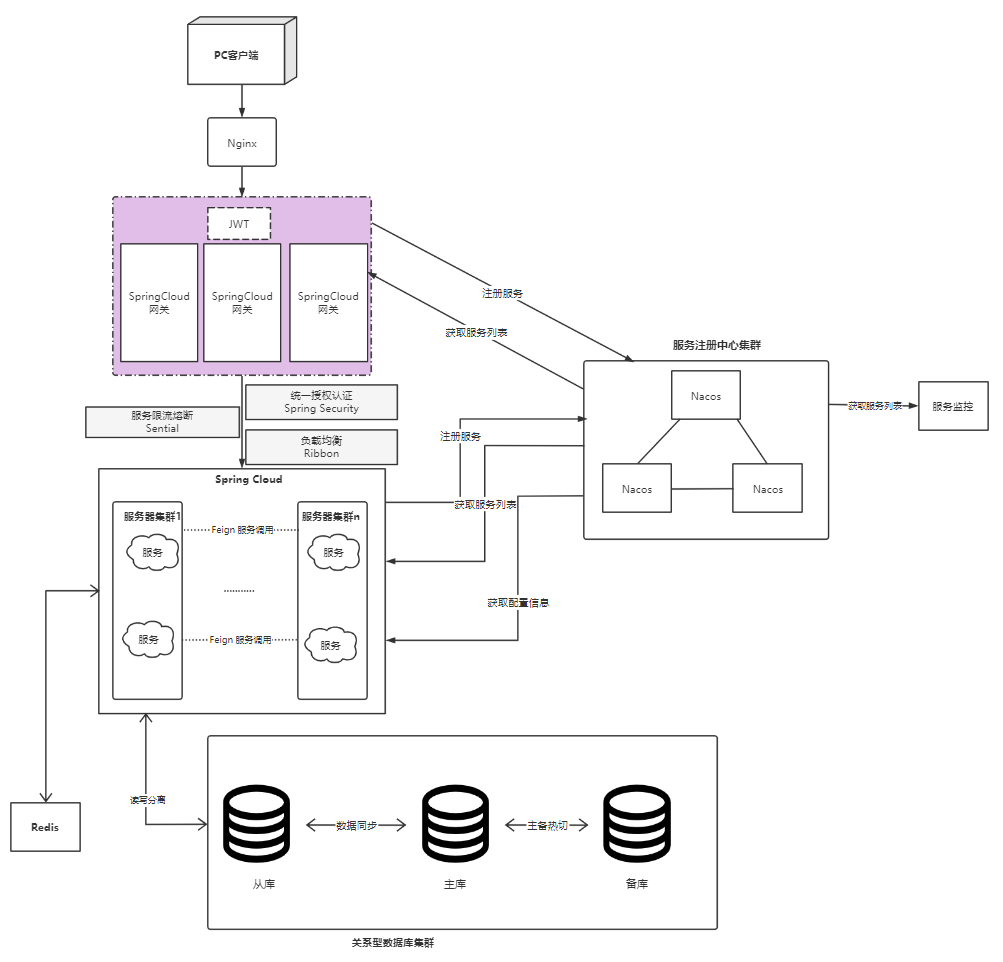
\includegraphics[width=\textwidth]{ch2/framework.png}
    \caption{总体架构}\label{fig:framework}
    \vspace{\baselineskip} % 表示图与正文空一行
\end{figure}

\subsection{具体微服务模块}
具体的微服务模块即系统给用户提供的业务服务,包括注册认证、发帖浏览等,每个具体微服务都整合了SpringCloud框架,微服务之间通过OpenFeign进行相互调用。
各个微服务集群部署,负载均衡技术采用ribbon,负载均衡策略为轮询。

\subsection{中间件}
本系统采用了许多微服务的中间件,以便更好地为微服务框架服务。
\subsubsection{服务注册与发现}
服务注册采用的是阿里巴巴开发的Nacos,部署方法为3个Nacos搭建服务注册集群。该集群可以实现各个微服务的注册,服务列表的获取和微服务的监听。
\subsubsection{服务调用}
本系统的服务调用技术采用的是OpenFeign,其为HTTP形式的REST API提供了简洁高效的RPC调用方式,同时OpenFeign也整合了负载均衡功能,便于集群之间的调用。
\subsubsection{负载均衡}
负载均衡技术使用的是Ribbon,结合OpenFeign实现微服务集群之间的互相调用,鉴于本系统的流量并不大,因此负载均衡策略采用轮询即可。
\subsubsection{网关}
网关技术使用的是Spring Gateway,他为众多服务模块提供了一个统一的访问路径,同时负责分发路由和认证授权,是所有服务调用的第一步。
\subsubsection{配置中心}
配置中心使用Nacos的配置中心,和Nacos服务注册中心紧密结合,将项目的配置文件进行统一的管理,同时也将项目的开发环境进行有效的隔离。
\subsubsection{服务降级和服务熔断}
本系统采用Sentinel技术实现服务降级和服务熔断,在流量超出服务器上限,或是出错率超过阈值时,会返回特定页面,以给客户更好的服务体验。
\subsubsection{消息队列}
本系统采用RabbitMQ实现消息队列,实现应用之间的异步调用,使得一些不需要及时反馈的操作可以异步进行,从而加快响应速度,提高用户体验。


\subsection{存储与缓存}
\subsubsection{数据库}
系统采用的为MySQL数据库,其数据模型的具体请详见后面的详细设计,会将每张数据表的字段和约束具体描述。
\subsubsection{缓存}
系统采用的是Redis缓存,其是基于内存的非关系型数据库,用于为本系统提升查询速度,主要在认证授权模块等高频模块使用。



\chapter{高层设计}
通过全局,虽然我们对该系统采用的是微服务架构,但是纵向来说,对于某个具体的模块,我们依然采用传统的MVC模式,即区分视图层、业务层和持久层。
视图层负责和前端进行数据交互,业务层负责业务逻辑处理,持久层负责和数据库进行数据交互,三层各司其职,实现系统的可控、可扩展。本章针对需求规格说明书提出
的需求进行提炼,给出本系统的层次结构,包括包图、部署图等设计。

\section{模块图}
系统中我们分为了许多Modules,主要为4个模块,Common、Service、GateWay、NacosCore,其作用分别是通用工具模块,微服务业务模块,网管模块和服务注册中心模块,
下面图~\ref{fig:Modules}~给出了系统的总体模块图。
\begin{figure}[htbp]
    \centering
    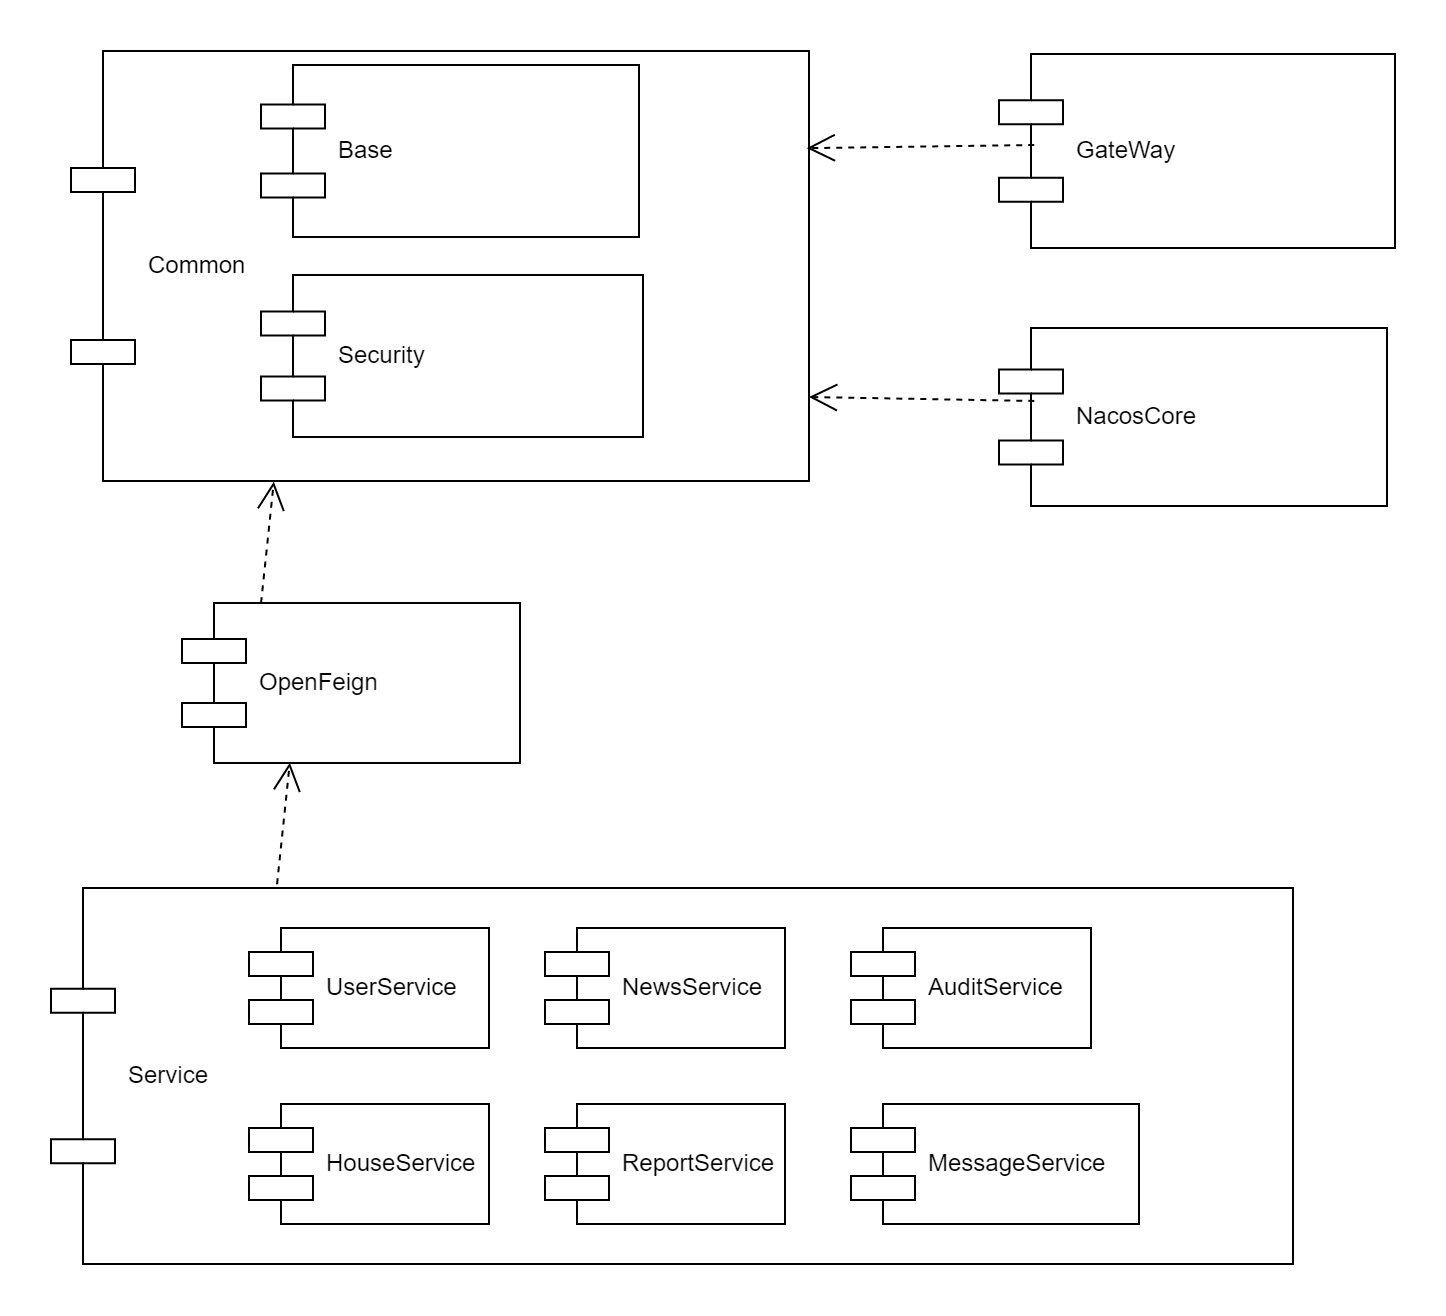
\includegraphics[width=\textwidth]{ch3/Modules.jpg}
    \caption{模块图}\label{fig:Modules}
    \vspace{\baselineskip} % 表示图与正文空一行
\end{figure}

其中四个模块还含有不同的子模块,我们对于四个模块的作用及其子模块做一个大致说明。
\begin{itemize}
    \item Common通用工具模块,将其他模块通用的功能抽象成一个独立的模块,便于调用。
    \begin{itemize}
        \item Base模块,包含了一些基本配置,比如Redis缓存的配置,返回类的配置等等。
        \item Security模块,整合了SpringSecurity框架,用于对用户进行认证授权。
    \end{itemize}
    \item Service微服务业务模块,即负责系统实际业务的模块,将所有业务统一到一个父类模块下,便于统一配置。
    \begin{itemize}
        \item UserService模块,负责处理用户信息的模块,包括用户登录、用户注册、管理获取用户列表等。
        \item HouseService模块,负责处理房源帖子的信息,包括发帖、改贴、帖子列表等。
        \item ReportService模块,负责举报信息,包括发起举报,审核举报等。
        \item NewsService模块,负责管理新闻信息,包括编辑新闻,获取新闻列表等。
        \item AuditService模块,负责管理审核信息,包括举报审核、新闻审核等。
        \item SystemService模块,负责处理系统的消息和系统业务对象,用于管理员给用户群发通知,业务对象管理等。
    \end{itemize}
    \item GateWay网管模块,负责分发路由,将请求转发到对应的微服务上,同时也负责初步校验JWT,检验用户身份。
    \item NacosCore微服务注册中心模块,负责管理系统中的各项微服务,包括服务注册、服务发现、流量监控等。
\end{itemize}

\section{包图}
接下来我们来设计各个模块中的包结构,不同功能的模块有着不同的包结构。大体来说,业务模块主要以MVC模式为主,即不同的层次对应不同的包,而配置相关的模块则
会根据配置类别进行不同的分包。

\subsection{Common通用工具模块}
Common模块中包含两个子模块,为Base模块和Security模块。
\subsubsection{Base}
Base中主要包含两个包,分别是Config和Util,分别负责一些全局参数的配置。Config中包含了Redis、RestTemplate、Constant(全局常量)的配置。Util中包含了ResponseUtil(统一返回设置)、Result(统一返回类)等全局统一用的配置。
Base模块的总体包图如图~\ref{fig:Base}~所示。
\begin{figure}[htbp]
    \centering
    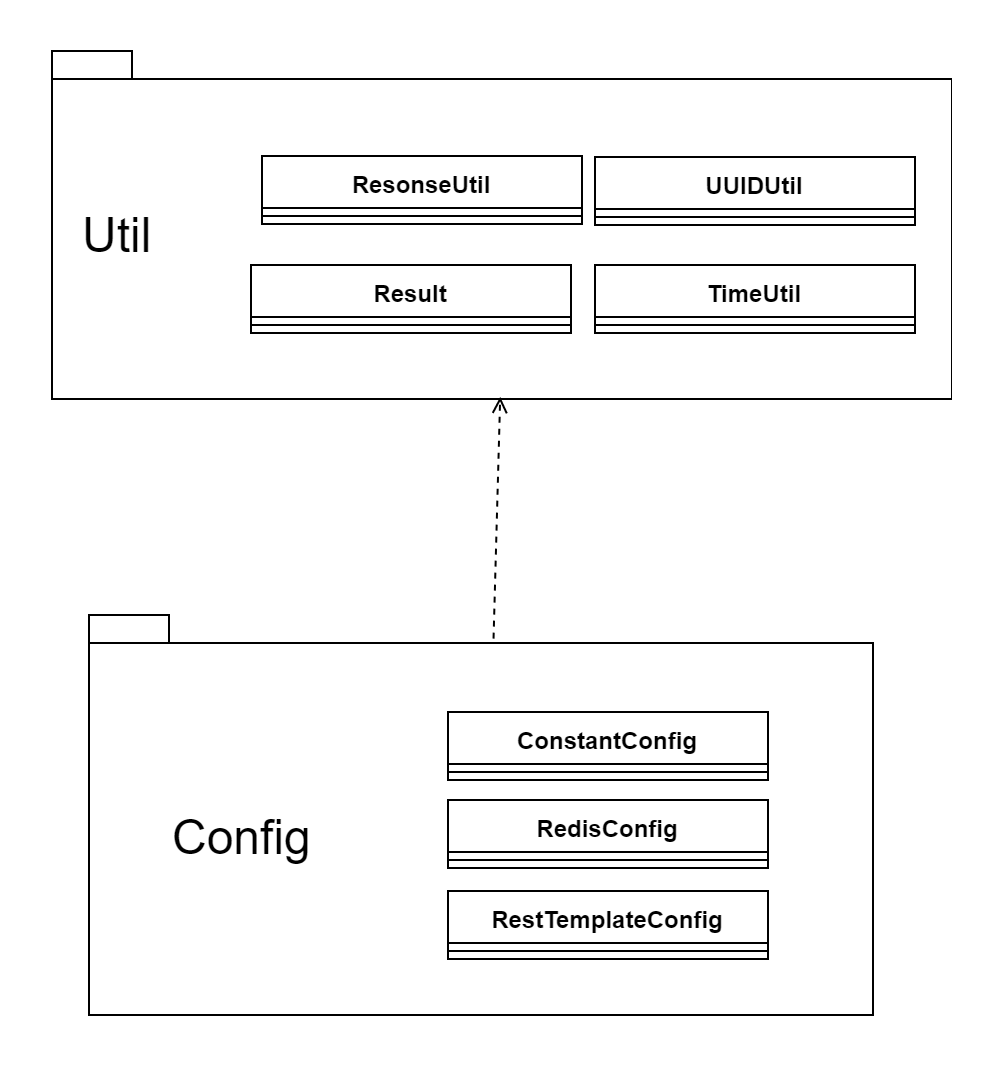
\includegraphics[width=0.6\textwidth]{ch3/Base.jpg}
    \caption{Base模块包图}\label{fig:Base}
    \vspace{\baselineskip} % 表示图与正文空一行
\end{figure}

\subsubsection{Security}
Security中主要包含4个包,为Config、Filter、Entity、Security。其中,Config为安全框架的具体配置,Filter中自定了一些过滤器,Entity中定义了一些实体类,Security中定义了具体的认证授权操作类。
Security模块的总体包图如图~\ref{fig:Security}~所示。
\begin{figure}[htbp]
    \centering
    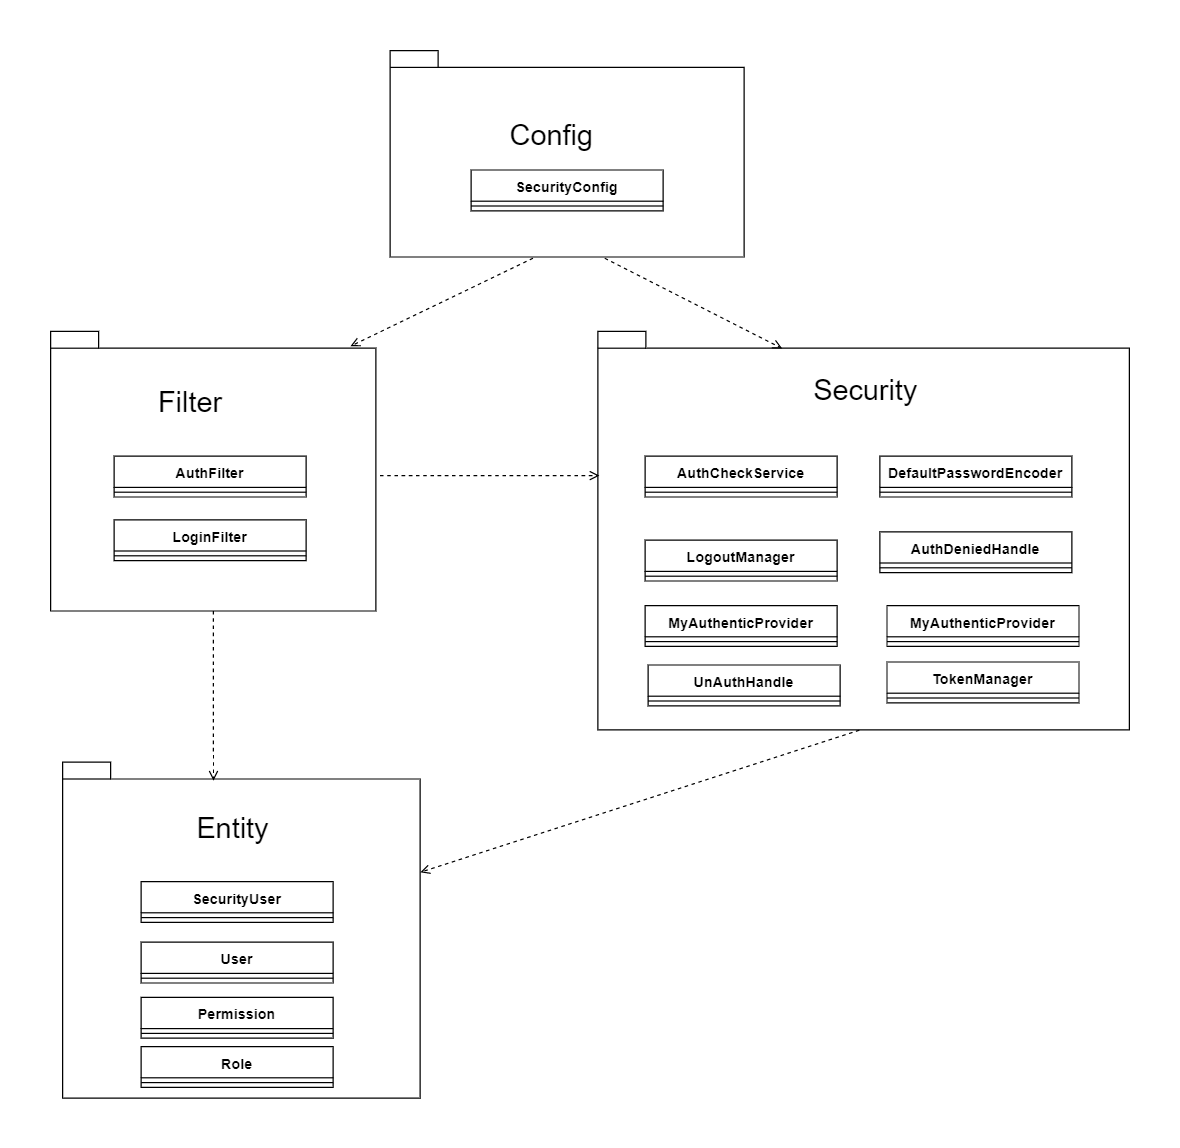
\includegraphics[width=\textwidth]{ch3/Security.jpg}
    \caption{Security模块包图}\label{fig:Security}
    \vspace{\baselineskip} % 表示图与正文空一行
\end{figure}

\subsection{Service微服务业务模块}
Service模块包含6个子模块,为UserService模块、HouseService模块、NewsService模块、ReportService模块、AuditService模块、SystemService模块。

\subsubsection{UserService}
UserService模块主要包含6个包,主要是MVC模式下的几个包,包括Controller、Service、Impl、Dao、Entity、Vo。前5个包的功能在前文均有描述,而Vo包的主要
功能是统一该模块的前端传来的数据模型,比如UserForm,以及后端返回给前端的数据模型,比如UserVo。
UserService模块的总体包图如图~\ref{fig:UserService}~所示。
\begin{figure}[htbp]
    \centering
    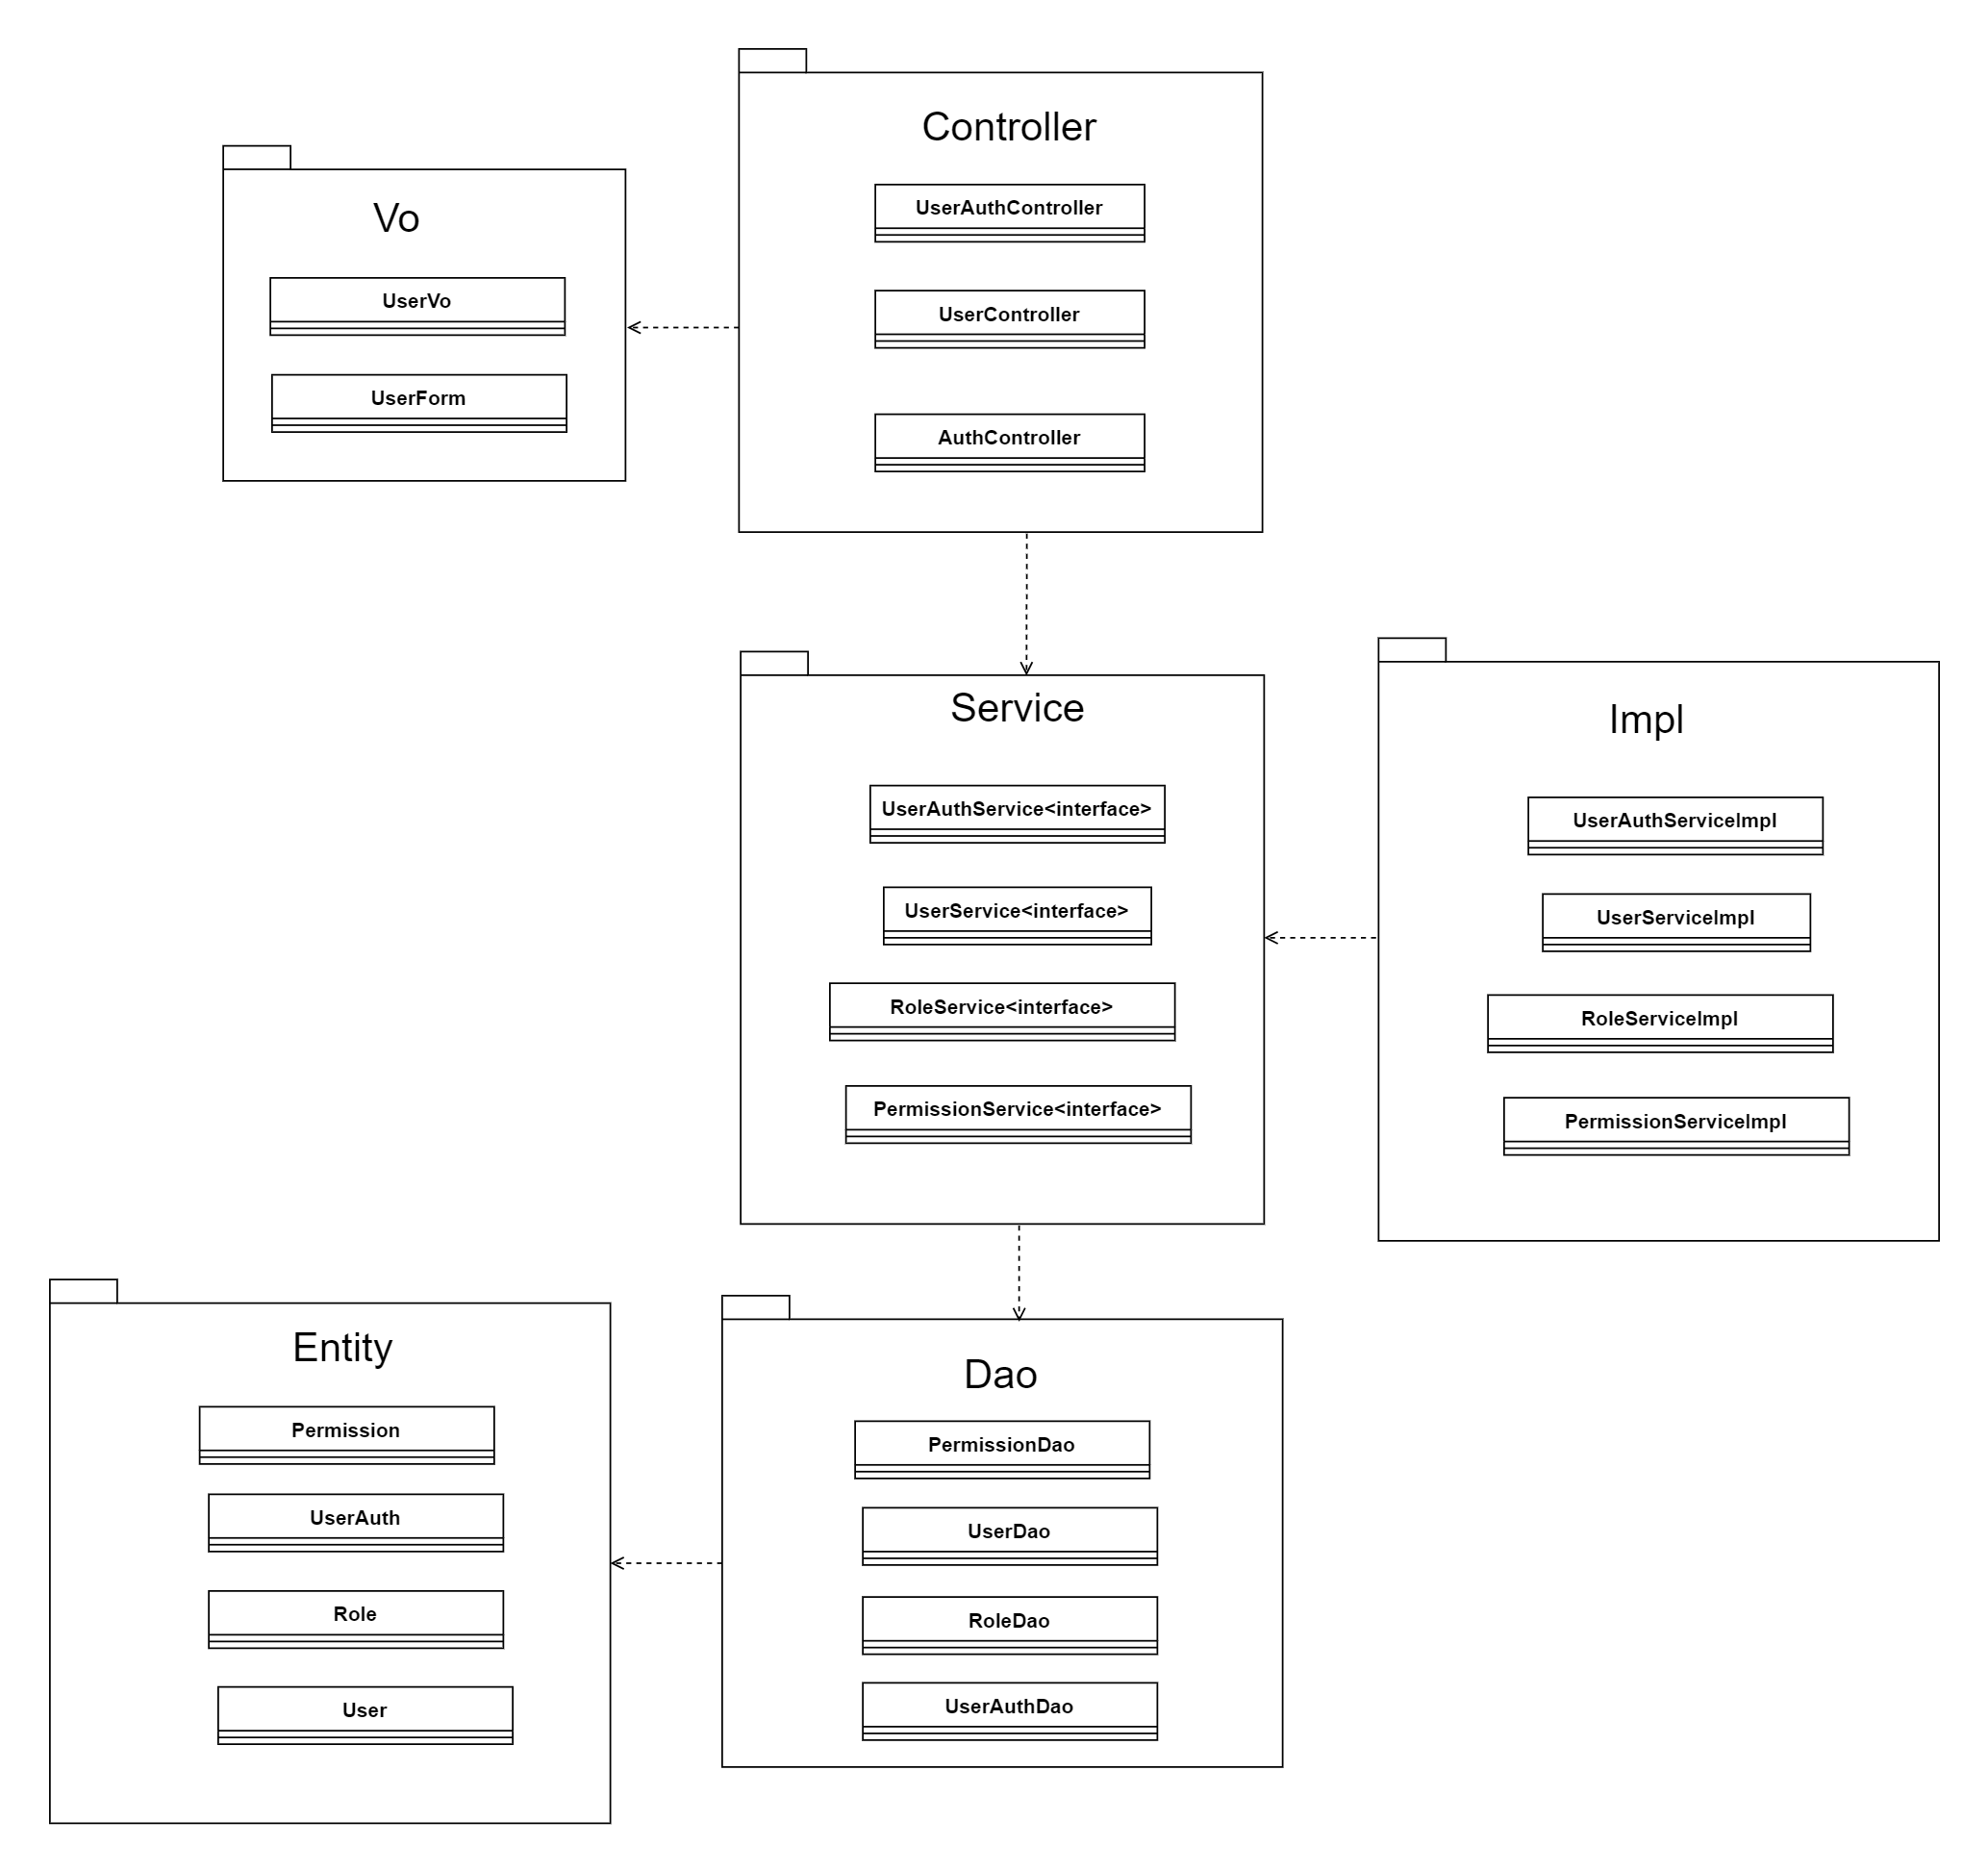
\includegraphics[width=\textwidth]{ch3/UserService.png}
    \caption{UserService模块包图}\label{fig:UserService}
    \vspace{\baselineskip} % 表示图与正文空一行
\end{figure}


\subsubsection{HouseService}
HouseService模块和上文一样,也包含6个包。总体包图如图所示。
\begin{figure}[htbp]
    \centering
    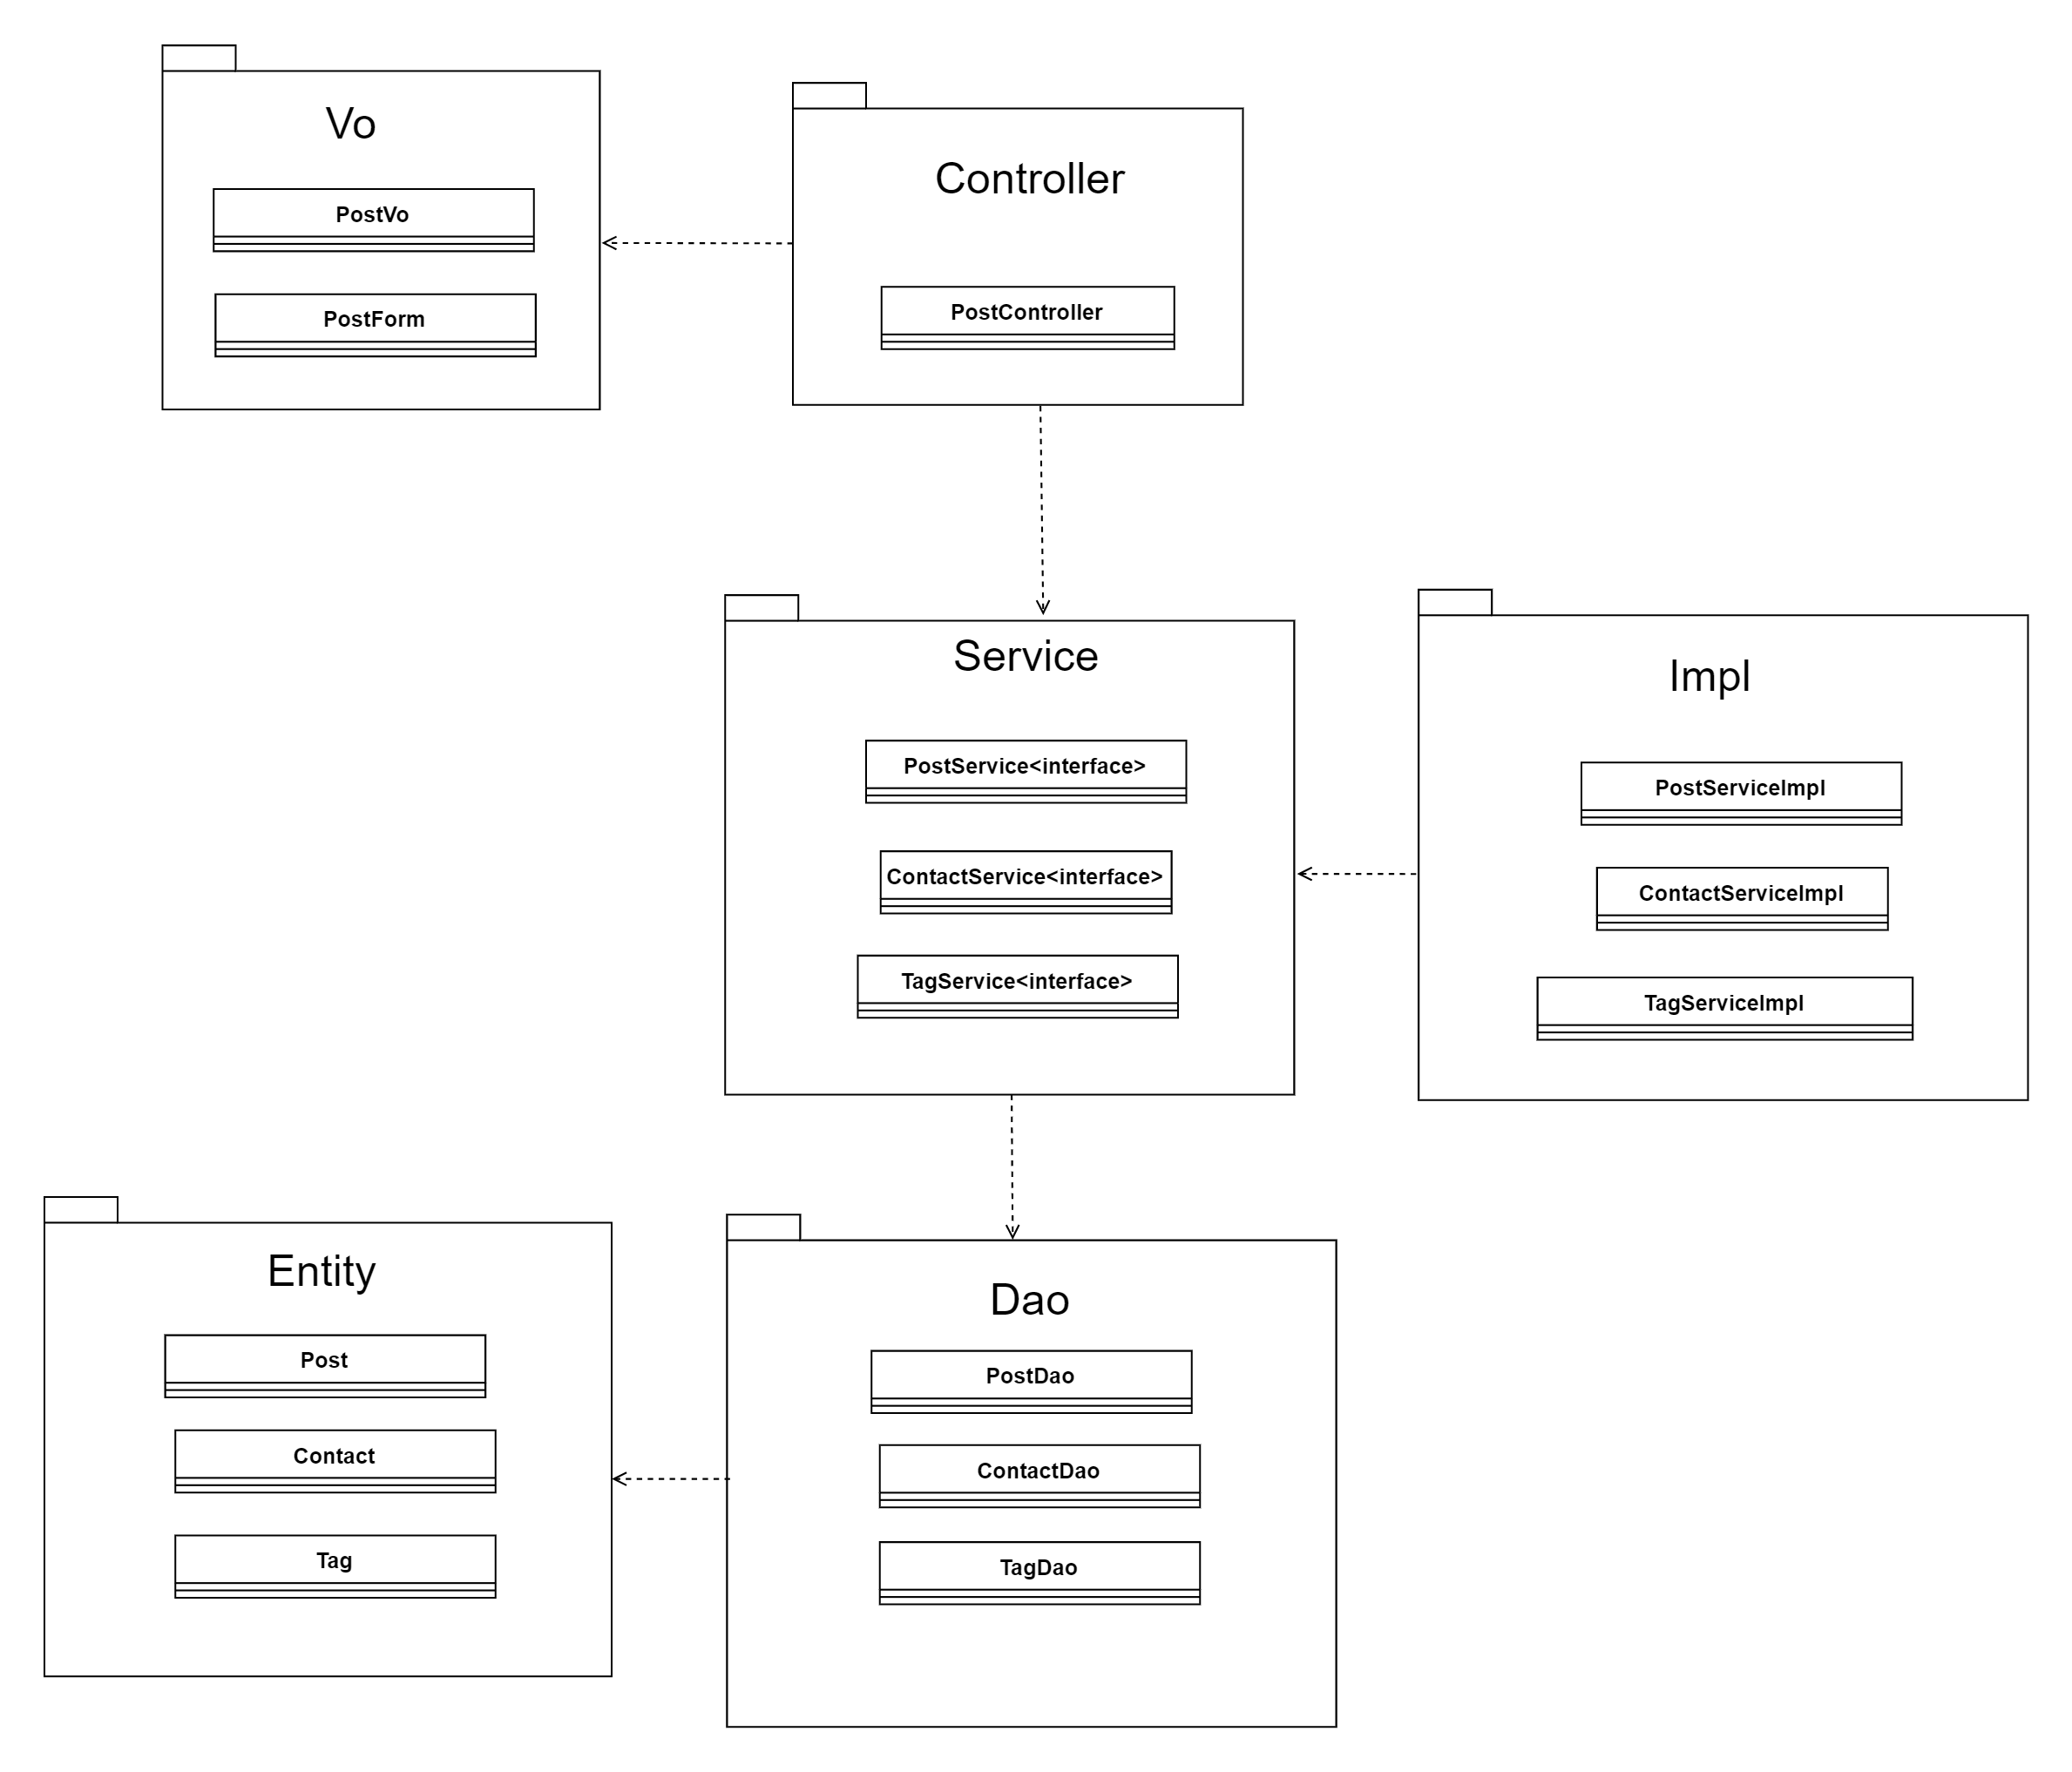
\includegraphics[width=\textwidth]{ch3/HouseService.jpg}
    \caption{HouseService模块包图}\label{fig:HouseService}
    \vspace{\baselineskip} % 表示图与正文空一行
\end{figure}

\subsubsection{NewsService}
包含6个包,总体包图如图~\ref{fig:NewsService}~所示。
\begin{figure}[htbp]
    \centering
    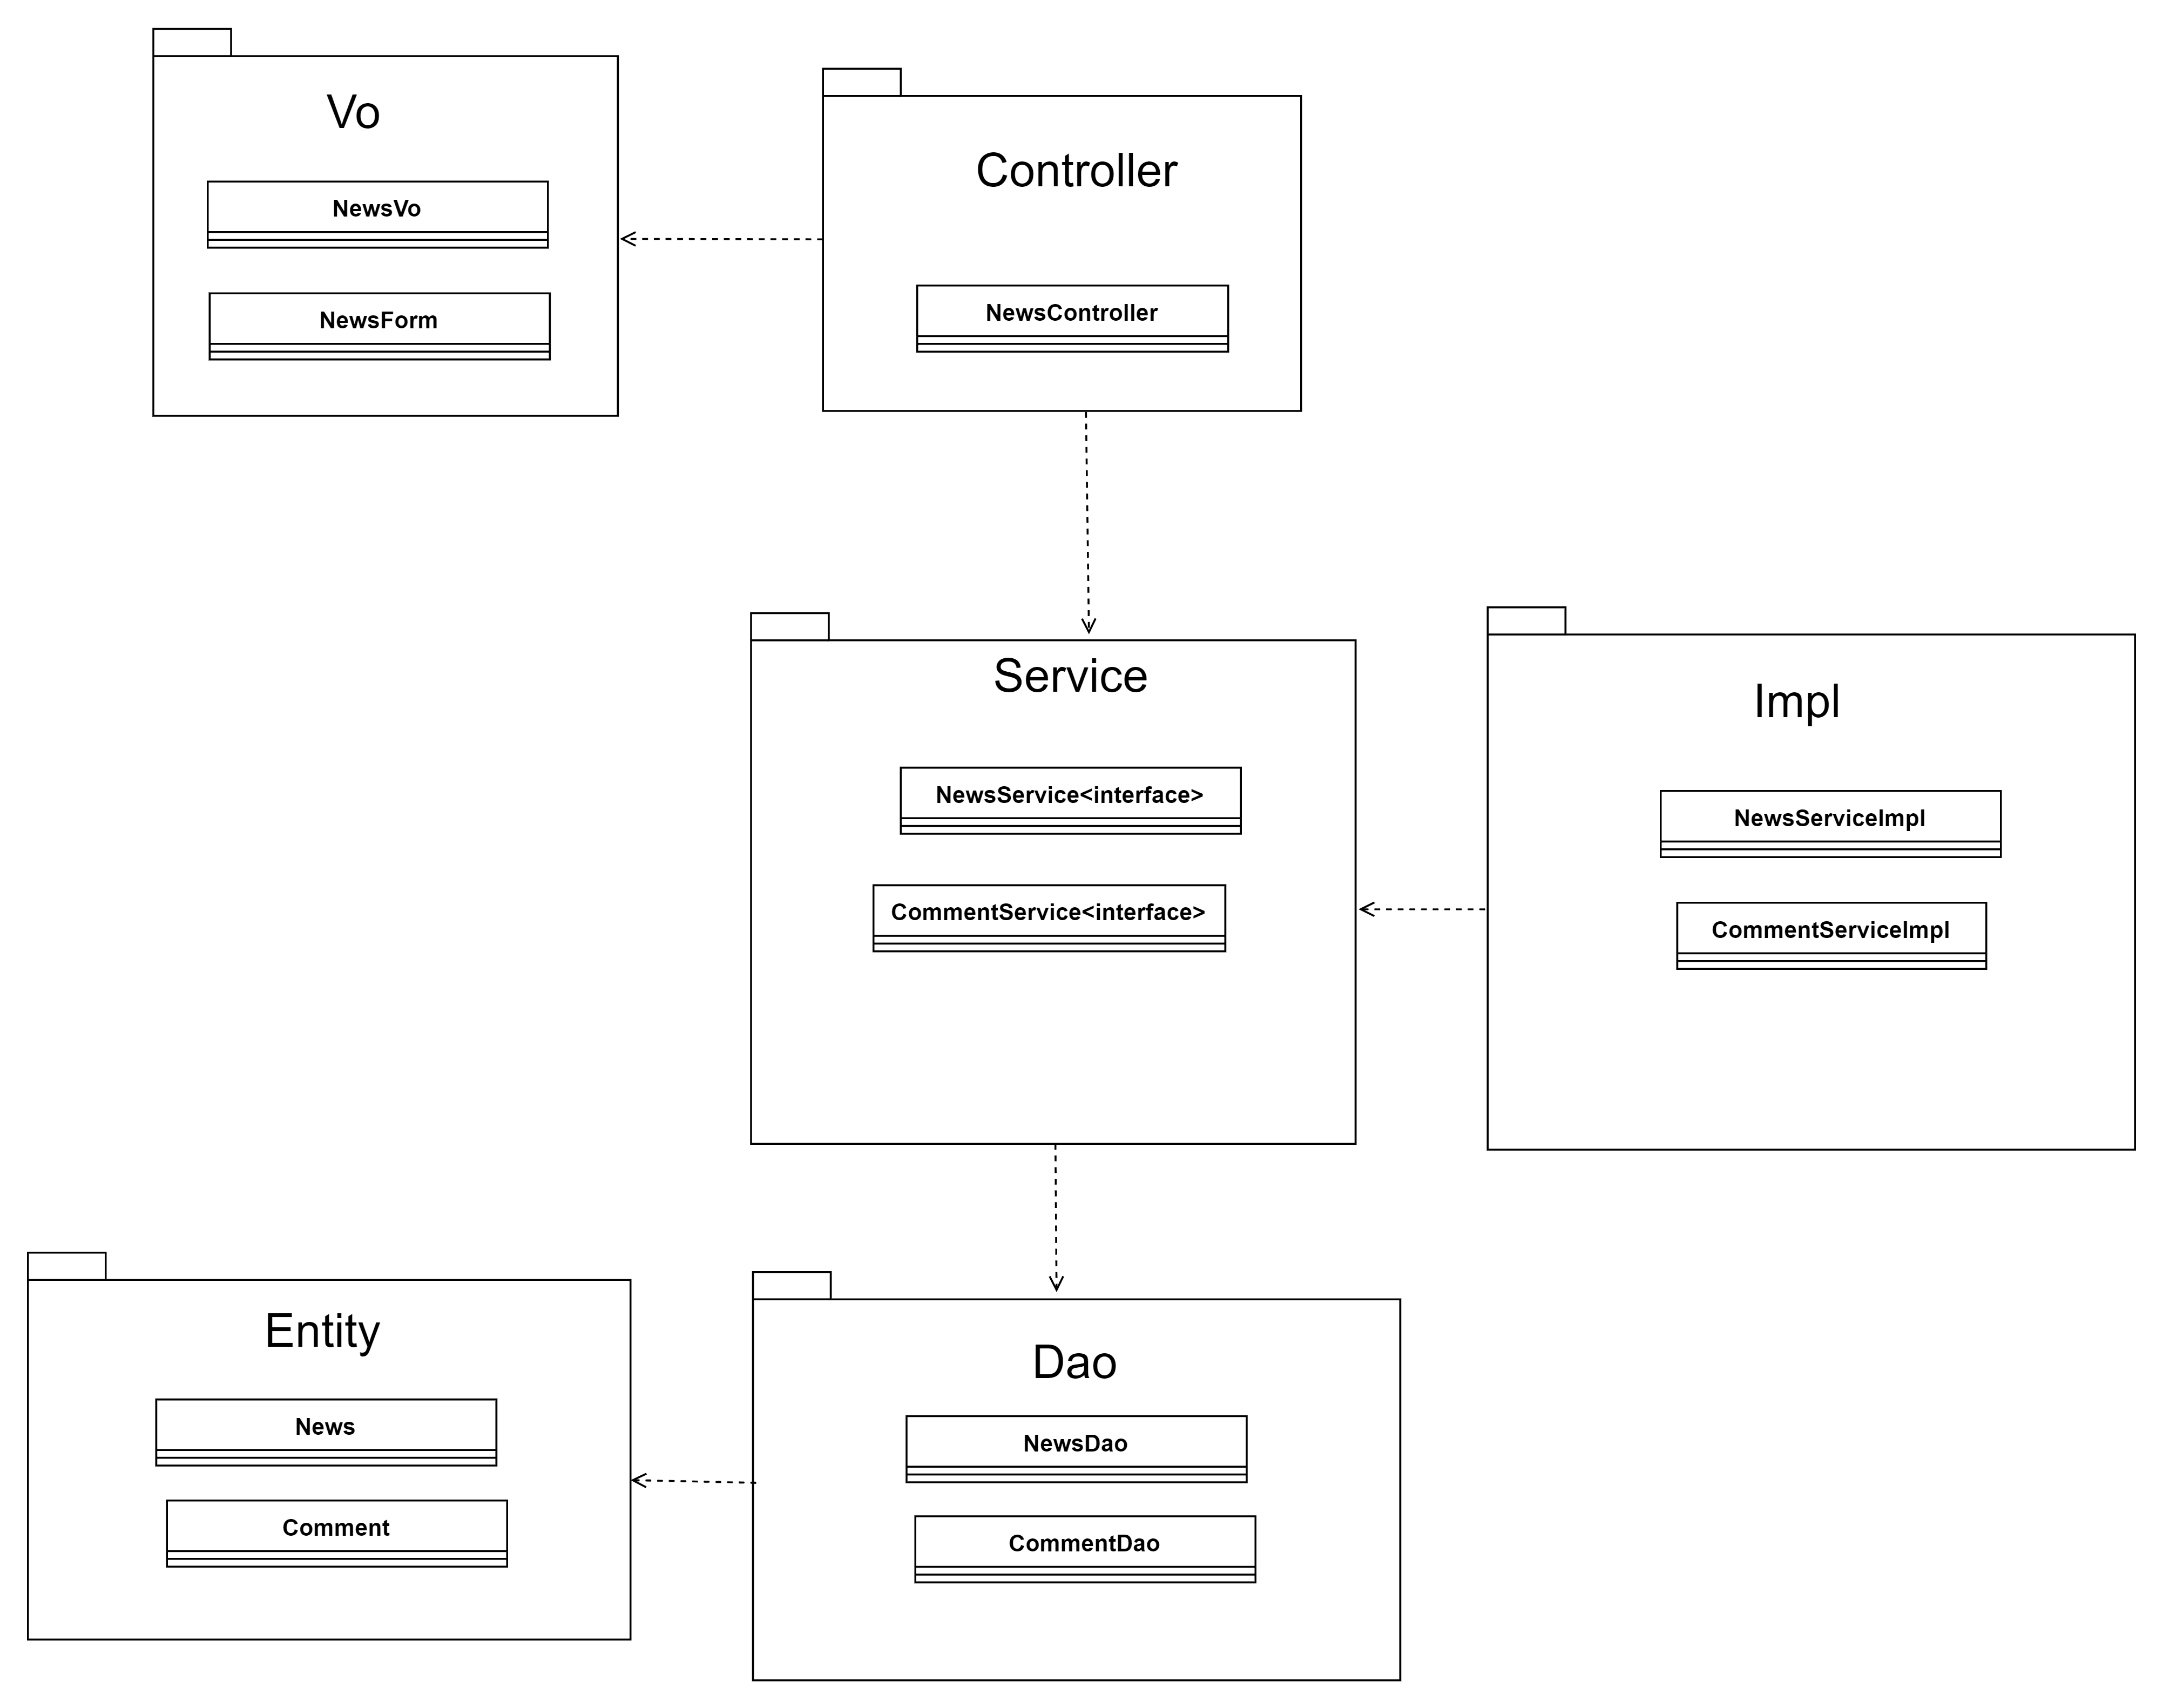
\includegraphics[width=\textwidth]{ch3/NewsService.jpg}
    \caption{NewsService模块包图}\label{fig:NewsService}
    \vspace{\baselineskip} % 表示图与正文空一行
\end{figure}

\subsubsection{ReportService}
包含6个包,总体包图如图~\ref{fig:ReportService}~所示。
\begin{figure}[htbp]
    \centering
    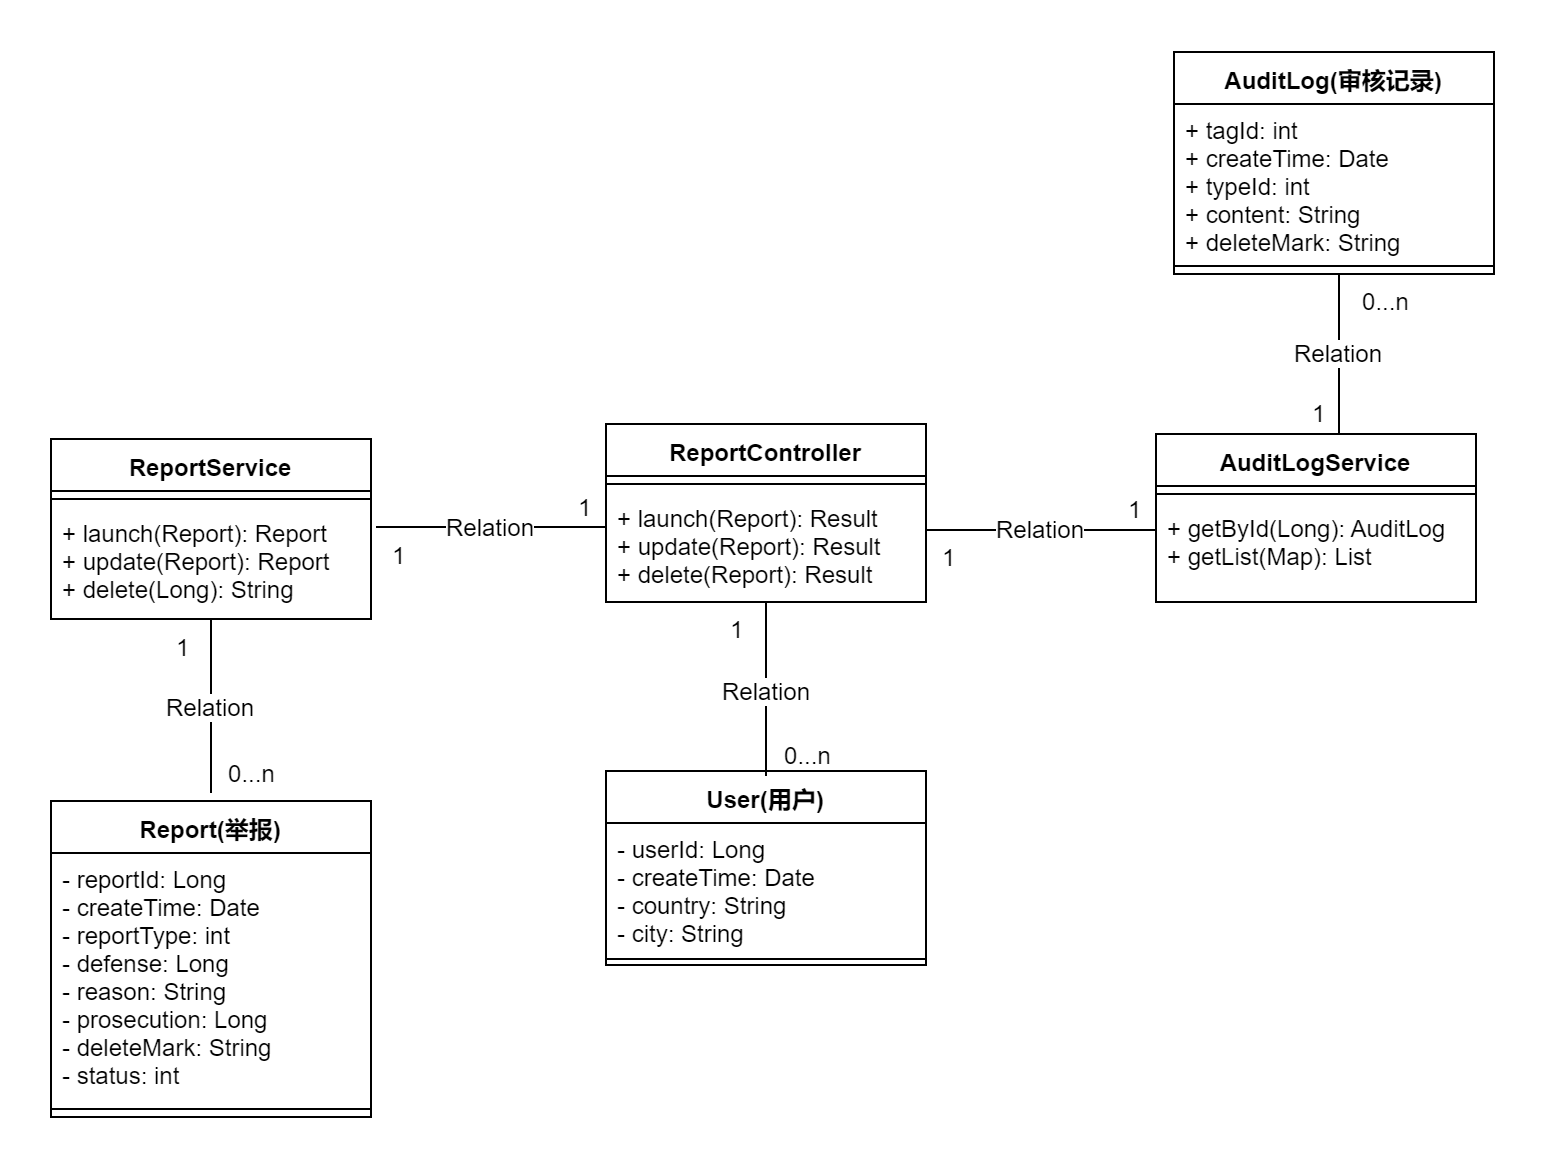
\includegraphics[width=\textwidth]{ch3/ReportService.jpg}
    \caption{ReportService模块包图}\label{fig:ReportService}
    \vspace{\baselineskip} % 表示图与正文空一行
\end{figure}

\subsubsection{AuditService}
包含6个包,总体包图如图~\ref{fig:AuditReport}~所示。
\begin{figure}[htbp]
    \centering
    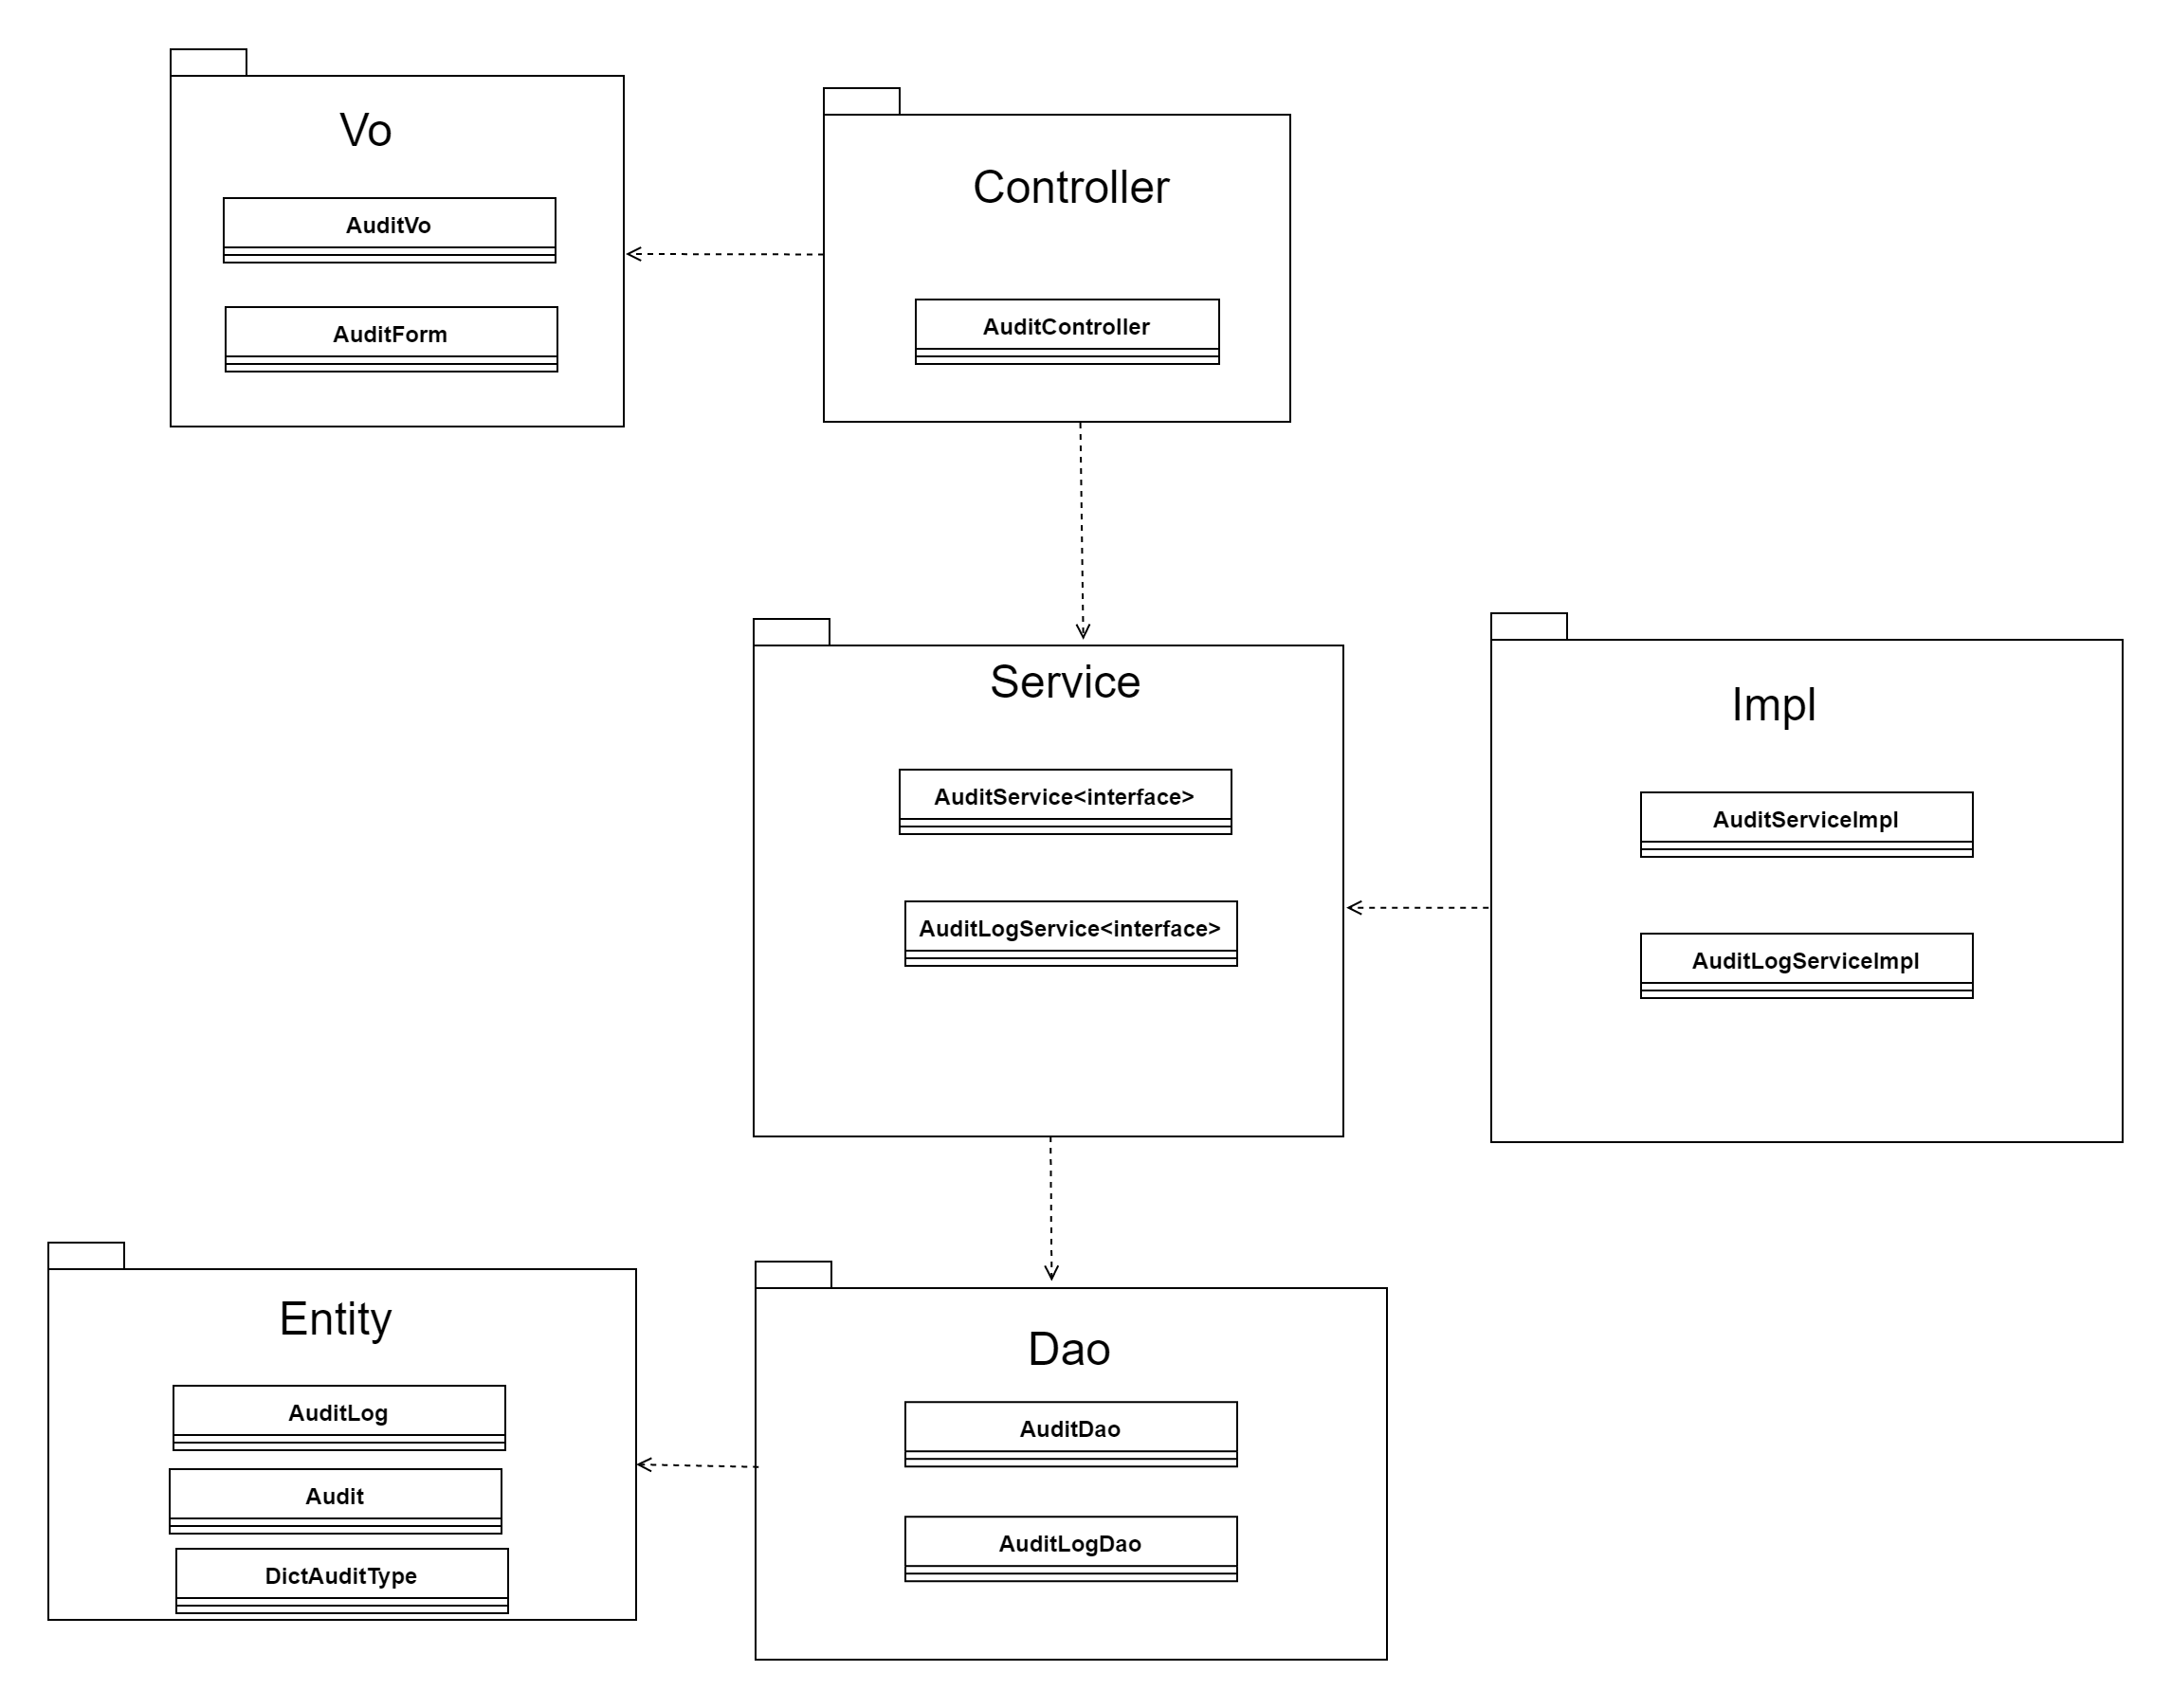
\includegraphics[width=\textwidth]{ch3/AuditService.jpg}
    \caption{AuditService模块包图}\label{fig:AuditService}
    \vspace{\baselineskip} % 表示图与正文空一行
\end{figure}

\subsubsection{SystemService}
总体包图如图~\ref{fig:SystemService}~所示。
\begin{figure}[htbp]
    \centering
    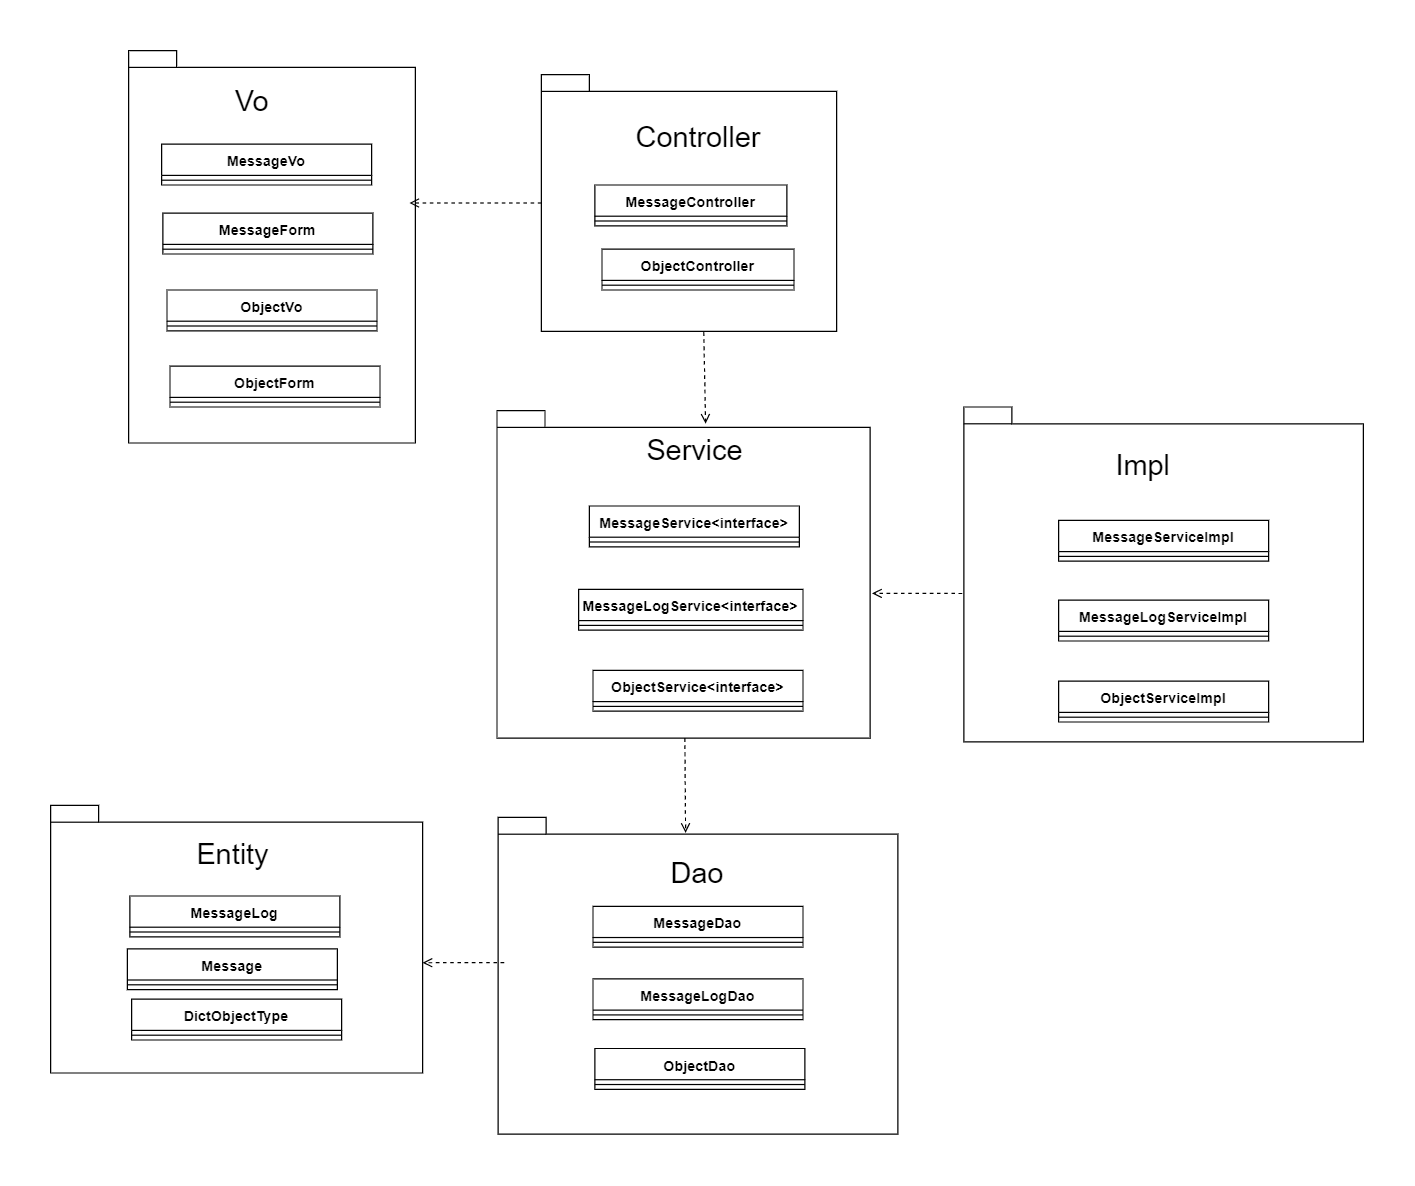
\includegraphics[width=\textwidth]{ch3/SystemService.jpg}
    \caption{SystemService模块包图}\label{fig:SystemService}
    \vspace{\baselineskip} % 表示图与正文空一行
\end{figure}


\subsection{GateWay网关模块}
GateWay网关模块负责路由转发,同时还负责初步的用户权限检查。所谓的网关权限检查,即对于用户的登陆凭证token进行初步检验。由于路由转发功能在配置文件中
已经实现,需要自定义的权限检查只需要一个包即可。下面为GateWay网关模块的包图~\ref{fig:GateWay}~。
\begin{figure}[htbp]
    \centering
    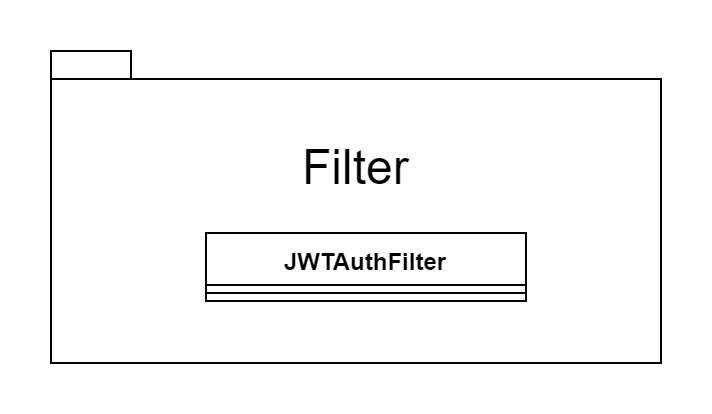
\includegraphics[width=0.7\textwidth]{ch3/GateWay.jpg}
    \caption{GateWay模块包图}\label{fig:GateWay}
    \vspace{\baselineskip} % 表示图与正文空一行
\end{figure}

\subsection{系统部署图}
本系统的部署主要涉及到服务端、客户端和数据库。客户端主要为Web浏览器,服务端需要部署多个微服务,同时启动Redis服务,数据库使用MySQL数据库。
系统部署图如图~\ref{fig:goujian}~所示。
\begin{figure}[htbp]
    \centering
    \includegraphics[width=\textwidth]{ch3/goujian.png}
    \caption{系统部署图}\label{fig:goujian}
    \vspace{\baselineskip} % 表示图与正文空一行
\end{figure}
\chapter{接口说明}
本章将对系统中的应用的接口,包括interface,abstract class进行详细说明,主要在于说明他们的public方法,以及方法中参数的意义和返回值的意义。

\section{Security模块}
为了便于扩展不同的认证授权方案,Security模块定义了许多认证授权操作的接口,以及相关过滤器的抽象类,包括登录过滤器、授权过滤器、用户加载接口等。
\subsection{UsernamePasswordAuthenticationFilter}
此抽象类为登录时调用的过滤器类。类中共定义了3个主要方法,作用分别为用户认证、认证成功和认证失败。
\begin{itemize}
    \item attemptAuthentication方法,返回类型为Authentication(用户认证类),参数有2个,类型分别为HttpServletRequest、HttpServletResponse。方法用途为将request中的用户信息进行校验。
    \item successfulAuthentication方法,返回类型为void,参数有4个,类型分别为HttpServletRequest、HttpServletResponse、Authentication、FilterChain(过滤链)。方法用途为用户认证成功后进行相关操作,包括加载权限等,然后将用户认证信息通过过滤链传递给下个过滤器。
    \item unsuccessfulAuthentication方法,返回类型为void,参数有3个,类型分别为HttpServletRequest、HttpServletResponse、Authentication。方法用途为用户认证失败后进行相关操作,包括返回失败信息等。
\end{itemize}

\subsection{BasicAuthenticationFilter}
此抽象类为授权时调用的过滤器类,类中需要说明的方法主要有1个,作用是获取用户权限,然后交给鉴权过滤器去鉴权。
\begin{itemize}
    \item doFilterInternal方法,返回类型为void,参数有3个,类型分别为HttpServletRequest、HttpServletResponse、FilterChain。方法用途为将request中的用户进行权限加载,然后把权限信息交给鉴权过滤器去鉴权。
\end{itemize}

\subsection{AccessDeniedHandler}
此接口定义了用户权限不够时所调用方法。主要的方法有1个,作用是设置用户权限不足的信息,然后将其返回给用户。
\begin{itemize}
    \item handle方法,返回类型为void,参数有3个,类型分别为HttpServletRequest、HttpServletResponse、AccessDeniedException(权限异常类)。方法用途为在HttpServletResponse中设置用户权限不足的信息并返回给用户。
\end{itemize}

\subsection{AuthenticationEntryPoint}
此接口定义了用户认证失败时所调用方法。主要的方法有1个,作用是设置用户认证失败的信息,然后将其返回给用户。
\begin{itemize}
    \item commence方法,返回类型为void,参数有3个,类型分别为HttpServletRequest、HttpServletResponse、AuthenticationException(认证异常类)。方法用途为在HttpServletResponse中设置用户认证失败的信息并返回给用户。
\end{itemize}

\subsection{PasswordEncoder}
此接口定义了用户密码加密和匹配的策略,主要有2个方法,作用分别是用户密码的加密算法和用户密码的匹配算法。
\begin{itemize}
    \item encode方法,返回类型为String,参数有1个,类型为CharSequence(用户传来的原始密码),作用在于对用户输入的密码进行加密计算,至于加密密码可以自定义,比如md5加密等。
    \item matches方法,返回类型为Boolean,参数有2个,类型都是CharSequence,分别表示用户输入的密码和数据库查询的密码,然后通过自定义的匹配算法进行匹配。
\end{itemize}

\subsection{UserDetailsService}
此接口定义了用户详细信息的加载方法,主要是1个方法,作用为从数据库加载用户的基本信息、角色信息和权限信息,并进行用户登录初始化工作。
\begin{itemize}
    \item loadUserByUsername方法,返回类型为UserDetail,参数有1个,类型分别为String,表示登录用户的用户名。方法用途为根据传入的用户名从数据库加载用户基本信息、角色信息和权限信息,并进行初始化工作,比如权限信息存入Redis缓存等。
\end{itemize}

\section{GateWay模块}
因为GateWay网关是需要处理客户端发来的一切请求,我们需要自定义一些过滤器。为了可扩展性,需要一个全局的过滤器类,实现过滤器的扩展。
\subsection{GlobalFilter}
此接口定义了过滤器实际过滤采用的方法,主要方法有1个,作用是接收并预处理客户端发来的一切请求。
\begin{itemize}
    \item filter方法,返回类型为Mono<void>,参数有2个,类型分别为ServerWebExchange(客户端请求)、GatewayFilterChain(网关过滤器链)。方法用途为将客户端请求进行预处理,如果符合要求则放行,否则返回错误信息。
\end{itemize}

\section{Service模块}
Service是业务模块,用的是MVC的框架,其中将每个具体的业务方法都进行了interface+impl的组合,即每个业务方法都被抽象成了一个接口,这样的话
我们需要进行扩展就只需要新建impl即可,增加了系统的可扩展性。


\chapter{功能性需求}
\section{执行者分析}
各个执行者的关系如图~\ref{fig:roleRelation}所示。

在本项目中一共有四个角色,分别是难民,房主,编辑员和管理员。

房主继承难民,难民的所有功能房主都能拥有。难民即是游客,无需登陆注册就可以查看信息。游客想要成为房主需要注册登录并且完成实名认证才能够进行房源的发布,这是为了保障信息的真实有效性,来帮助更多的难民。
否则则默认是难民(游客)。

编辑员和管理员都属于管理层角色。编辑员拥有所有游客(难民)的基本功能,但是不能发布房源,因为编辑员默认没有登陆注册,只是有编辑新闻页面的权限,这里体现了权限管理。
管理者是系统中的权限最高的人物,所以同时拥有编辑员的所有权限,因此管理员继承自编辑员,但是拥有发布房源等救助信息、管理用户权限、管理角色权限的权限。

所以得到如图\ref{fig:roleRelation}所示的执行者关系图。
\begin{figure}[htbp]
    \centering
    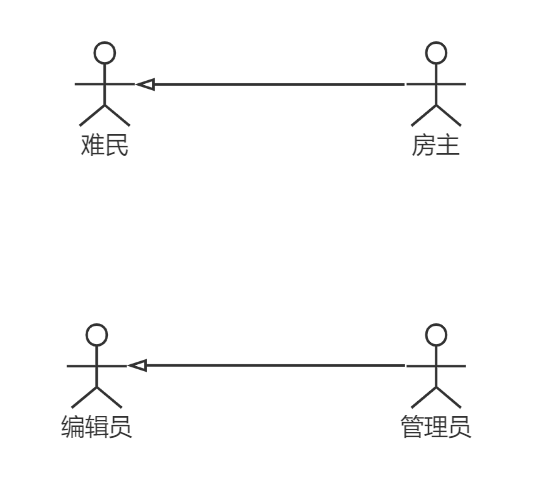
\includegraphics[width=0.8\textwidth]{ch5/roleRelation.png}
    \caption{执行者关系图}\label{fig:roleRelation}
    \vspace{\baselineskip} % 表示图与正文空一行
\end{figure}

\section{总用例图}
总用例图如图~\ref{fig:overallUseCase}~所示,其中包含了所有角色在系统中的功能,并且对于每一种角色这里只给出\textbf{第一层的用例图},详细的用例图会在接下来4个小节中详细介绍。

\begin{figure}[htbp]
    \centering
    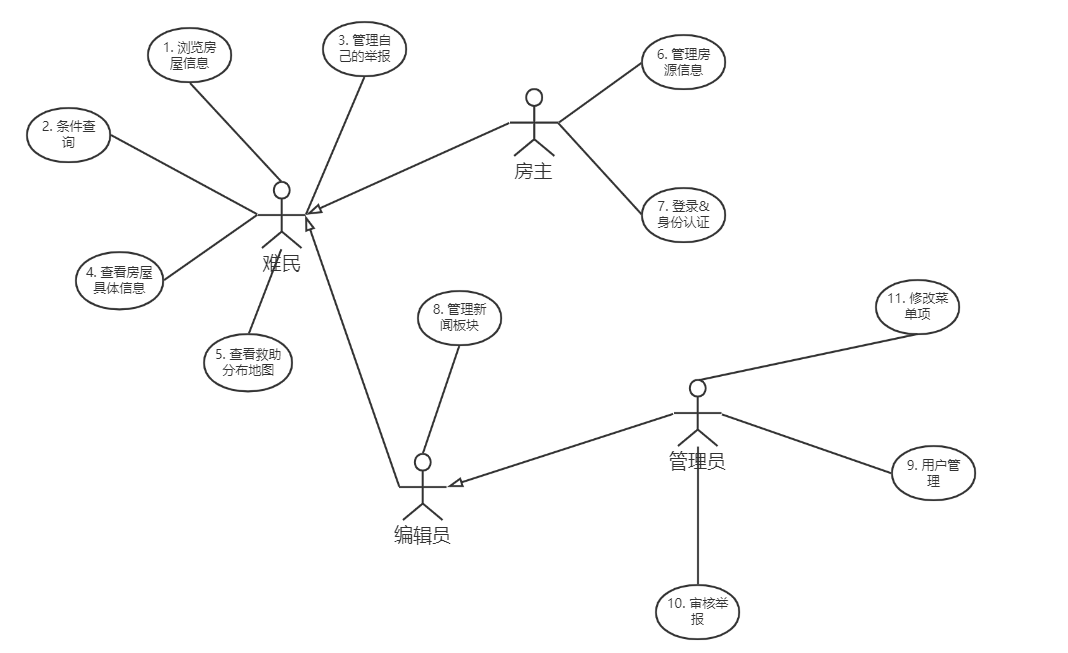
\includegraphics[width=\textwidth]{ch5/overallUseCase.png}
    \caption{总用例图}\label{fig:overallUseCase}
    \vspace{\baselineskip} % 表示图与正文空一行
\end{figure}

\section{难民用例图}

难民的用例图如图~\ref{fig:refugeeUseCase}~所示。

\begin{figure}[htbp]
    \centering
    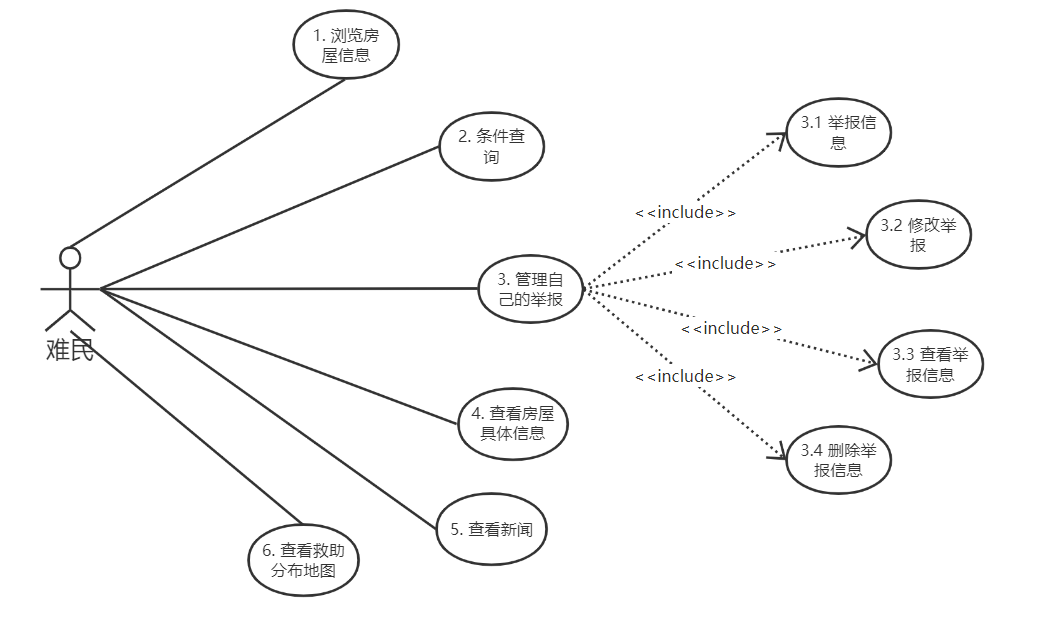
\includegraphics[width=0.8\textwidth]{ch5/refugeeUseCase.png}
    \caption{难民用例图}\label{fig:refugeeUseCase}
    \vspace{\baselineskip} % 表示图与正文空一行
\end{figure}

% 1 浏览房屋信息
\begin{table}[htbp]
    \centering
    \caption{浏览房屋信息}
    \vspace{0.5em}\wuhao
    \begin{tabular}{|l|l|l|l|}
        \hline
        \makebox[0.12\textwidth][l]{编号} & \makebox[0.25\textwidth][c]{UC-01 1}                      & \makebox[0.15\textwidth][l]{名称} & \makebox[0.3\textwidth][c]{浏览房屋信息} \\
        \hline
        执行者                            & \makebox[0.25\textwidth][c]{\makecell[c]{难民\quad房主                                                                                   \\编辑员\quad管理员}} & 优先级                            & \makebox[0.3\textwidth][c]{高 ~$\blacksquare$ ~中 ~$\square$~ 低 ~$\square$~} \\
        \hline
        描述                              & \multicolumn{3}{l|}{
        \begin{minipage}[t]{0.8\linewidth}
                目标:

                难民能够在浏览房主发布的房源信息概要和基本信息,选择匹配的房源。

                具体要求:

                \begin{enumerate}[nosep]
                    \item 难民能看到具有简要信息的房源信息。
                    \item 房源信息需要按照发布时间逆序排列。
                    \item 房源信息以卡片的形式展现,需要展示如地址,入住要求等基本信息。
                    \item 需要有分页或者加载更多按钮来展现更多数据。
                          \vspace{0.5em}
                \end{enumerate}
            \end{minipage}     }                                                                                                                                             \\
        \hline
        前置条件                          & \multicolumn{3}{l|}{  房主发布房源信息并且录入数据库。  }                                                                                \\
        \hline
        基本流程                          & \multicolumn{3}{l|}{
        \begin{minipage}[t]{0.8\textwidth}
                \begin{enumerate}[nosep]
                    \item 进入房源信息页,查看信息。
                    \item 点击加载更多展示更多数据。
                          \vspace{0.5em}
                \end{enumerate}
            \end{minipage}     }                                                                                                                                             \\
        \hline
        结束状况                          & \multicolumn{3}{l|}{系统的数据不会发生变化。    }                                                                                        \\
        \hline
        可选流程                          & \multicolumn{3}{l|}{点击加载更多来展示更多数据。  }                                                                                      \\
        \hline
        异常流程                          & \multicolumn{3}{l|}{暂时没有可用的房源信息。    }                                                                                        \\
        \hline
        说明                              & \multicolumn{3}{l|}{无     }                                                                                                             \\
        \hline
    \end{tabular}
\end{table}

% 2 条件查询
\begin{table}[htbp]
    \centering
    \caption{条件查询}
    \vspace{0.5em}\wuhao
    \begin{tabular}{|l|l|l|l|}
        \hline
        \makebox[0.12\textwidth][l]{编号} & \makebox[0.25\textwidth][c]{UC-01 2}                      & \makebox[0.15\textwidth][l]{名称} & \makebox[0.3\textwidth][c]{条件查询} \\
        \hline
        执行者                            & \makebox[0.25\textwidth][c]{\makecell[c]{难民\quad房主                                                                               \\编辑员\quad管理员}}                       & 优先级                            & \makebox[0.3\textwidth][c]{高 ~$\blacksquare$ ~中 ~$\square$~ 低 ~$\square$~} \\
        \hline
        描述                              & \multicolumn{3}{l|}{
        \begin{minipage}[t]{0.8\linewidth}
                目标: 难民通过过滤器找到符合自己要求的房源等救助信息。
                \vspace{0.5em}
            \end{minipage}     }                                                                                                                                          \\
        \hline
        前置条件                          & \multicolumn{3}{l|}{  房主发布房源信息并且录入数据库。  }                                                                            \\
        \hline
        基本流程                          & \multicolumn{3}{l|}{
        \begin{minipage}[t]{0.8\textwidth}
                \begin{enumerate}[nosep]
                    \item 难民通过过滤器筛选条件。
                    \item 提交查询结果。
                    \item 显示查询成功并返回查询结果。
                          \vspace{0.5em}
                \end{enumerate}
            \end{minipage}     }                                                                                                                                         \\
        \hline
        结束状况                          & \multicolumn{3}{l|}{系统的数据不会发生变化。    }                                                                                    \\
        \hline
        可选流程                          & \multicolumn{3}{l|}{点击加载更多来展示更多数据。  }                                                                                  \\
        \hline
        异常流程                          & \multicolumn{3}{l|}{暂时没有相关的房源信息。 }                                                                                       \\
        \hline
        说明                              & \multicolumn{3}{l|}{无     }                                                                                                         \\
        \hline
    \end{tabular}
\end{table}

% 3 举报信息
\begin{table}[htbp]
    \centering
    \caption{举报信息}
    \vspace{0.5em}\wuhao
    \begin{tabular}{|l|l|l|l|}
        \hline
        \makebox[0.12\textwidth][l]{编号} & \makebox[0.25\textwidth][c]{UC-01 3-1}                                                           & \makebox[0.15\textwidth][l]{名称} & \makebox[0.3\textwidth][c]{举报信息}                                          \\
        \hline
        执行者                            & \makebox[0.25\textwidth][c]{难民\quad 房主}                                                      & 优先级                            & \makebox[0.3\textwidth][c]{高 ~$\blacksquare$ ~中 ~$\square$~ 低 ~$\square$~} \\
        \hline
        描述                              & \multicolumn{3}{l|}{\makecell[l]{难民/房主对于虚假不合规、房主违反提供住宿承诺的房源信息可以进行                                                                                                                     \\举报。}    }                                                                                                                     \\
        \hline
        前置条件                          & \multicolumn{3}{l|}{  房主发布房源信息并且录入数据库。难民能够看到房源信息。  }                                                                                                                                      \\
        \hline
        基本流程                          & \multicolumn{3}{l|}{
        \begin{minipage}[t]{0.8\textwidth}
                \begin{enumerate}[nosep]
                    \item 指示新建举报。
                    \item 显示举报申请表。
                    \item 填写申请单,选择请假类别。
                    \item 指示提交申请。
                    \item 显示成功提交申请的信息。
                          \vspace{0.5em}
                \end{enumerate}
            \end{minipage}     }                                                                                                                                                                                                                         \\
        \hline
        结束状况                          & \multicolumn{3}{l|}{系统保存举报的具体信息,并返回数据成功录入数据库的结果。    }                                                                                                                                    \\
        \hline
        可选流程                          & \multicolumn{3}{l|}{\begin{minipage}[t]{0.8\textwidth}
                \begin{enumerate}[nosep]
                    \item 指示取消举报。
                    \item 显示举报取消的信息。
                          \vspace{0.5em}
                \end{enumerate}
            \end{minipage}  }                                                                                                                                                                    \\
        \hline
        异常流程                          & \multicolumn{3}{l|}{   无}                                                                                                                                                                                           \\
        \hline
        说明                              & \multicolumn{3}{l|}{举报提交之后需要等待管理员审核并返回举报结果。    }                                                                                                                                              \\
        \hline
    \end{tabular}
\end{table}

% 4 修改举报信息
\begin{table}[htbp]
    \centering
    \caption{修改举报信息}
    \vspace{0.5em}\wuhao
    \begin{tabular}{|l|l|l|l|}
        \hline
        \makebox[0.12\textwidth][l]{编号} & \makebox[0.25\textwidth][c]{UC-01 3-2}                                                    & \makebox[0.15\textwidth][l]{名称} & \makebox[0.3\textwidth][c]{修改举报信息}                                      \\
        \hline
        执行者                            & \makebox[0.25\textwidth][c]{难民\quad 房主 \quad 编辑员}                                  & 优先级                            & \makebox[0.3\textwidth][c]{高 ~$\blacksquare$ ~中 ~$\square$~ 低 ~$\square$~} \\
        \hline
        描述                              & \multicolumn{3}{l|}{
        \begin{minipage}[t]{0.8\textwidth}
                目标:

                难民/房主/编辑员对于虚假不合规、房主违反提供住宿承诺的房源信息和不实的新闻可以进行举报。

                具体要求:

                \begin{enumerate}[nosep]
                    \item 举报申请提出以后,还没有任何审核之前,申请者可以修改请假申请。
                    \item 举报信息如果没有通过,申请者可以修改请假申请,重新提交。
                    \item 举报信息结果会以消息的形式发送到用户提交的联系方式中。
                          \vspace{0.5em}
                \end{enumerate}
            \end{minipage}     }                                                                                                                                                                                                                  \\
        \hline
        前置条件                          & \multicolumn{3}{l|}{  需存在已提交的举报信息。  }                                                                                                                                                             \\
        \hline
        基本流程                          & \multicolumn{3}{l|}{
        \begin{minipage}[t]{0.8\textwidth}
                \begin{enumerate}[nosep]
                    \item 查看自己的举报信息。
                    \item 点击某一具体举报信息的修改按钮。
                    \item 重新输入举报信息。
                    \item 重新提交。
                          \vspace{0.5em}
                \end{enumerate}
            \end{minipage}     }                                                                                                                                                                                                                  \\
        \hline
        结束状况                          & \multicolumn{3}{l|}{系统保存新提交的举报的具体信息,并返回数据成功录入数据库的结果。    }                                                                                                                     \\
        \hline
        可选流程                          & \multicolumn{3}{l|}{\begin{minipage}[t]{0.8\textwidth}
                \begin{enumerate}[nosep]
                    \item 指示取消举报。
                    \item 显示举报取消的信息。
                          \vspace{0.5em}
                \end{enumerate}
            \end{minipage}  }                                                                                                                                                             \\
        \hline
        异常流程                          & \multicolumn{3}{l|}{   无}                                                                                                                                                                                    \\
        \hline
        说明                              & \multicolumn{3}{l|}{举报提交之后需要等待管理员审核并返回举报结果。    }                                                                                                                                       \\
        \hline
    \end{tabular}
\end{table}

% 5 查看举报信息
\begin{table}[htbp]
    \centering
    \caption{查看举报信息}
    \vspace{0.5em}\wuhao
    \begin{tabular}{|l|l|l|l|}
        \hline
        \makebox[0.12\textwidth][l]{编号} & \makebox[0.25\textwidth][c]{UC-01 3-3}                   & \makebox[0.15\textwidth][l]{名称} & \makebox[0.3\textwidth][c]{查看举报信息}                                      \\
        \hline
        执行者                            & \makebox[0.25\textwidth][c]{难民\quad 房主 \quad 编辑员} & 优先级                            & \makebox[0.3\textwidth][c]{高 ~$\blacksquare$ ~中 ~$\square$~ 低 ~$\square$~} \\
        \hline
        描述                              & \multicolumn{3}{l|}{
        \begin{minipage}[t]{0.8\textwidth}
                目标:

                可以方便的查看自己的举报信息的审核情况,能查看自己的历史申请,在此基础上做下一步工作。

                具体要求:

                \begin{enumerate}[nosep]
                    \item 系统按照默认时间逆序显示当前用户的请假申请列表,用户可以通过该列表查看各举报的状态。
                    \item 举报申请可以按照时间的倒序或顺序排列,也可以按照举报的状态进行筛选。
                    \item 在查看申请的时候,角色可以查看或修改其中的一个具体的申请,或提出举报申请。
                    \item 用户在查看一个具体申请的时候才能删除该举报申请。
                          \vspace{0.5em}
                \end{enumerate}
            \end{minipage}     }                                                                                                                                                                                 \\
        \hline
        前置条件                          & \multicolumn{3}{l|}{用户有举报记录。 }                                                                                                                                       \\
        \hline

        结束状况                          & \multicolumn{3}{l|}{系统的数据不会发生变化。  }                                                                                                                              \\
        \hline
        异常流程                          & \multicolumn{3}{l|}{   无}                                                                                                                                                   \\
        \hline
        说明                              & \multicolumn{3}{l|}{无    }                                                                                                                                                  \\
        \hline
    \end{tabular}
\end{table}

% 6 删除举报信息
\begin{table}[htbp]
    \centering
    \caption{删除举报信息}
    \vspace{0.5em}\wuhao
    \begin{tabular}{|l|l|l|l|}
        \hline
        \makebox[0.12\textwidth][l]{编号} & \makebox[0.25\textwidth][c]{UC-01 3-4}                   & \makebox[0.15\textwidth][l]{名称} & \makebox[0.3\textwidth][c]{删除举报信息}                                      \\
        \hline
        执行者                            & \makebox[0.25\textwidth][c]{难民\quad 房主 \quad 编辑员} & 优先级                            & \makebox[0.3\textwidth][c]{高 ~$\blacksquare$ ~中 ~$\square$~ 低 ~$\square$~} \\
        \hline
        描述                              & \multicolumn{3}{l|}{删除自己的举报信息。   }                                                                                                                                 \\
        \hline
        前置条件                          & \multicolumn{3}{l|}{  需存在已提交的举报信息。  }                                                                                                                            \\
        \hline
        基本流程                          & \multicolumn{3}{l|}{
        \begin{minipage}[t]{0.8\textwidth}
                \begin{enumerate}[nosep]
                    \item 查看举报历史信息。
                    \item 点击查看具体举报信息。
                    \item 删除举报信息。
                          \vspace{0.5em}
                \end{enumerate}
            \end{minipage}     }                                                                                                                                                                                 \\
        \hline
        结束状况                          & \multicolumn{3}{l|}{系统删除指定的举报信息。    }                                                                                                                            \\
        \hline
        可选流程                          & \multicolumn{3}{l|}{
        \begin{minipage}[t]{0.8\textwidth}
                \begin{enumerate}[nosep]
                    \item 指示取消删除举报。
                    \item 显示举报删除取消的信息。
                          \vspace{0.5em}
                \end{enumerate}
            \end{minipage}  }                                                                                                                                                                                    \\
        \hline
        异常流程                          & \multicolumn{3}{l|}{ \begin{minipage}[t]{0.8\textwidth}
                \begin{enumerate}[nosep]
                    \item 指示删除举报。
                    \item 显示该举报正在受理或已受理完毕,无法删除。
                    \item 取消删除。
                          \vspace{0.5em}
                \end{enumerate}
            \end{minipage}}                                                                                                                             \\
        \hline
        说明                              & \multicolumn{3}{l|}{无    }                                                                                                                                                  \\
        \hline
    \end{tabular}
\end{table}

% 7 查看房源具体信息
\begin{table}[htbp]
    \centering
    \caption{查看房源具体信息}
    \vspace{0.5em}\wuhao
    \begin{tabular}{|l|l|l|l|}
        \hline
        \makebox[0.12\textwidth][l]{编号} & \makebox[0.25\textwidth][c]{UC-01 4}                                 & \makebox[0.15\textwidth][l]{名称} & \makebox[0.3\textwidth][c]{查看房源具体信息}                                  \\
        \hline
        执行者                            & \makebox[0.25\textwidth][c]{难民\quad 房主 \quad 编辑员}             & 优先级                            & \makebox[0.3\textwidth][c]{高 ~$\blacksquare$ ~中 ~$\square$~ 低 ~$\square$~} \\
        \hline
        描述                              & \multicolumn{3}{l|}{
        \begin{minipage}[t]{0.8\textwidth}
                用户可以查看房源的具体信息。
            \end{minipage}     }                                                                                                                                                                                             \\
        \hline
        前置条件                          & \multicolumn{3}{l|}{  房主发布了房源。  }                                                                                                                                                \\
        \hline
        基本流程                          & \multicolumn{3}{l|}{
        \begin{minipage}[t]{0.8\textwidth}
                \begin{enumerate}[nosep]
                    \item 查看房源信息列表。
                    \item 点击查看具体房源信息。
                          \vspace{0.5em}
                \end{enumerate}
            \end{minipage}     }                                                                                                                                                                                             \\
        \hline
        结束状况                          & \multicolumn{3}{l|}{系统的数据不会发生任何变化。    }                                                                                                                                    \\
        \hline
        可选流程                          & \multicolumn{3}{l|}{无 }                                                                                                                                                                 \\
        \hline
        异常流程                          & \multicolumn{3}{l|}{无}                                                                                                                                                                  \\
        \hline
        说明                              & \multicolumn{3}{l|}{房源信息列表要有基本的信息如地址,接纳条件等。 }                                                                                                                     \\
        \hline
    \end{tabular}
\end{table}

% 8 查看新闻
\begin{table}[htbp]
    \centering
    \caption{查看新闻}
    \vspace{0.5em}\wuhao
    \begin{tabular}{|l|l|l|l|}
        \hline
        \makebox[0.12\textwidth][l]{编号} & \makebox[0.25\textwidth][c]{UC-01 5}                         & \makebox[0.15\textwidth][l]{名称} & \makebox[0.3\textwidth][c]{查看新闻}                                          \\
        \hline
        执行者                            & \makebox[0.25\textwidth][c]{难民\quad 房主 \quad 编辑员}     & 优先级                            & \makebox[0.3\textwidth][c]{高 ~$\blacksquare$ ~中 ~$\square$~ 低 ~$\square$~} \\
        \hline
        描述                              & \multicolumn{3}{l|}{
        \begin{minipage}[t]{0.8\textwidth}
                用户可以查看新闻的具体信息。
            \end{minipage}     }                                                                                                                                                                                     \\
        \hline
        前置条件                          & \multicolumn{3}{l|}{  编辑员发布了新闻。  }                                                                                                                                      \\
        \hline
        基本流程                          & \multicolumn{3}{l|}{
        \begin{minipage}[t]{0.8\textwidth}
                \begin{enumerate}[nosep]
                    \item 查看新闻信息列表。
                    \item 点击查看具体新闻信息。
                          \vspace{0.5em}
                \end{enumerate}
            \end{minipage}     }                                                                                                                                                                                     \\
        \hline
        结束状况                          & \multicolumn{3}{l|}{系统的数据不会发生任何变化。    }                                                                                                                            \\
        \hline
        可选流程                          & \multicolumn{3}{l|}{无 }                                                                                                                                                         \\
        \hline
        异常流程                          & \multicolumn{3}{l|}{无}                                                                                                                                                          \\
        \hline
        说明                              & \multicolumn{3}{l|}{新闻列表要有基本的信息如标题,时间等。 }                                                                                                                     \\
        \hline
    \end{tabular}
\end{table}

% 9 查看救助地图
\begin{table}[htbp]
    \centering
    \caption{查看救助地图}
    \vspace{0.5em}\wuhao
    \begin{tabular}{|l|l|l|l|}
        \hline
        \makebox[0.12\textwidth][l]{编号} & \makebox[0.25\textwidth][c]{UC-01 6}                     & \makebox[0.15\textwidth][l]{名称} & \makebox[0.3\textwidth][c]{查看救助地图}                                      \\
        \hline
        执行者                            & \makebox[0.25\textwidth][c]{难民\quad 房主 \quad 编辑员} & 优先级                            & \makebox[0.3\textwidth][c]{高 ~$\square$ ~中 ~$\blacksquare$~ 低 ~$\square$~} \\
        \hline
        描述                              & \multicolumn{3}{l|}{
        \begin{minipage}[t]{0.8\textwidth}
                附近的救助信息,这些信息会以图标的形式在用户所在地的周围标注出来。
                \vspace{.5em}
            \end{minipage}     }                                                                                                                                                                                 \\
        \hline
        前置条件                          & \multicolumn{3}{l|}{  允许GPS定位。  }                                                                                                                                       \\
        \hline
        基本流程                          & \multicolumn{3}{l|}{无   }                                                                                                                                                   \\
        \hline
        结束状况                          & \multicolumn{3}{l|}{系统的数据不会发生任何变化。    }                                                                                                                        \\
        \hline
        可选流程                          & \multicolumn{3}{l|}{无 }                                                                                                                                                     \\
        \hline
        异常流程                          & \multicolumn{3}{l|}{无}                                                                                                                                                      \\
        \hline
        说明                              & \multicolumn{3}{l|}{
        \begin{minipage}[t]{0.8\textwidth}
                地图可以放大缩小,拖动,点击展示基本信息但是无法跳转,可以通过展示的基本信息进行条件查询。
                \vspace{.5em}
            \end{minipage} }                                                                                                                                                                                     \\
        \hline
    \end{tabular}
\end{table}
\section{房主用例图}

房主的用例图如图~\ref{fig:ownerUseCase}~所示。

\begin{figure}[htbp]
    \centering
    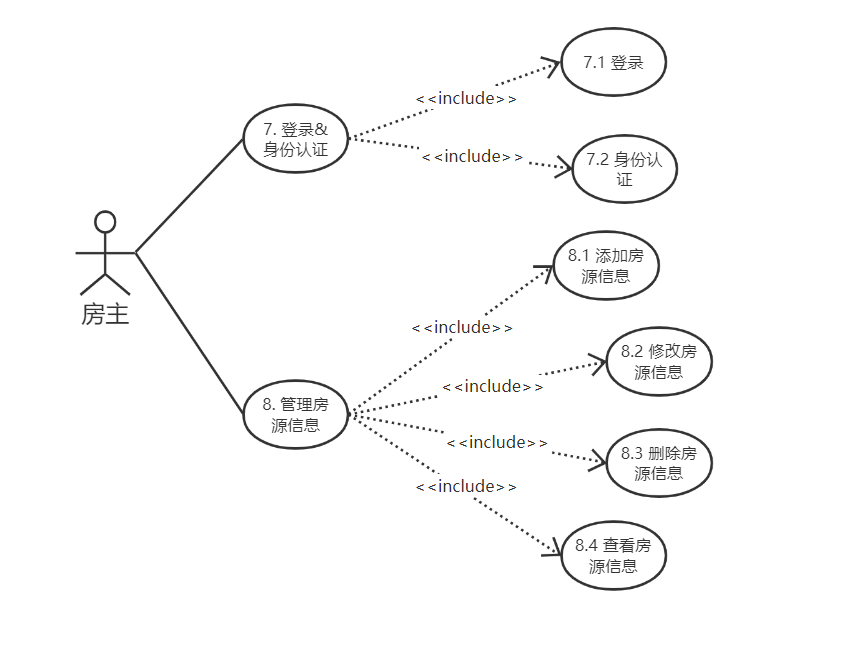
\includegraphics[width=.8\textwidth]{ch5/ownerUseCase.png}
    \caption{房主用例图}\label{fig:ownerUseCase}
    \vspace{\baselineskip} % 表示图与正文空一行
\end{figure}

% 10 登录
\begin{table}[htbp]
    \centering
    \caption{登录}
    \vspace{0.5em}\wuhao
    \begin{tabular}{|l|l|l|l|}
        \hline
        \makebox[0.12\textwidth][l]{编号} & \makebox[0.25\textwidth][c]{UC-02 7-1}                  & \makebox[0.15\textwidth][l]{名称} & \makebox[0.3\textwidth][c]{登录 \& 注册} \\
        \hline
        执行者                            & \makebox[0.25\textwidth][c]{\makecell[c]{难民\quad 房主                                                                                \\ 编辑员 \quad 管理员} }& 优先级                            & \makebox[0.3\textwidth][c]{高 ~$\blacksquare$ ~中 ~$\square$~ 低 ~$\square$~} \\
        \hline
        描述                              & \multicolumn{3}{l|}{部分功能需要用户登录才能操作。}                                                                                    \\
        \hline
        前置条件                          & \multicolumn{3}{l|}{  无  }                                                                                                            \\
        \hline
        基本流程                          & \multicolumn{3}{l|}{
            \begin{minipage}[t]{0.8\textwidth}
                \begin{enumerate}
                    \item 用户点击登录按钮。
                    \item 用户输入账号密码。
                    \item 登陆成功。
                \end{enumerate}
                \vspace{.5em}
            \end{minipage}
        }                                                                                                                                                                          \\
        \hline
        结束状况                          & \multicolumn{3}{l|}{数据库添加用户信息或改变状态。    }                                                                                \\
        \hline
        可选流程                          & \multicolumn{3}{l|}{无 }                                                                                                               \\
        \hline
        异常流程                          & \multicolumn{3}{l|}{
            \begin{minipage}[t]{0.8\textwidth}
                \begin{enumerate}
                    \item 账号密码没有输入,账号密码不匹配,用户名,密码不符合规范。
                    \item 弹出不规范提醒。
                    \item 重新登录或注册。
                \end{enumerate}
                \vspace{.5em}
            \end{minipage}
        }                                                                                                                                                                          \\
        \hline
        说明                              & \multicolumn{3}{l|}{
        \begin{minipage}[t]{0.8\textwidth}
                角色的有些功能需要登录,房主,编辑员和管理员必须登录。难民可以选择登录或者不登陆,如果难民不登陆,只能浏览房源信息,不能举报,查看举报信息等,此功能需要难民登录才能进行操作。
                \vspace{.5em}
            \end{minipage} }                                                                                                                                               \\
        \hline
    \end{tabular}
\end{table}

% 11 身份认证
\begin{table}[htbp]
    \centering
    \caption{身份认证}
    \vspace{0.5em}\wuhao
    \begin{tabular}{|l|l|l|l|}
        \hline
        \makebox[0.12\textwidth][l]{编号} & \makebox[0.25\textwidth][c]{UC-02 7-2}                        & \makebox[0.15\textwidth][l]{名称} & \makebox[0.3\textwidth][c]{身份认证} \\
        \hline
        执行者                            & \makebox[0.25\textwidth][c]{\makecell[c]{ 房主   \quad 编辑员                                                                            \\ 管理员} }& 优先级                            & \makebox[0.3\textwidth][c]{高 ~$\blacksquare$ ~中 ~$\square$~ 低 ~$\square$~} \\
        \hline
        描述                              & \multicolumn{3}{l|}{房主必须身份认证才能发布房源。}                                                                                      \\
        \hline
        前置条件                          & \multicolumn{3}{l|}{  无  }                                                                                                              \\
        \hline
        基本流程                          & \multicolumn{3}{l|}{
            \begin{minipage}[t]{0.8\textwidth}
                \begin{enumerate}
                    \item 点击be a host按钮
                    \item 依照提示上传ID证件
                    \item 认证完成
                \end{enumerate}
                \vspace{.5em}
            \end{minipage}
        }                                                                                                                                                                            \\
        \hline
        结束状况                          & \multicolumn{3}{l|}{数据库改变用户状态。    }                                                                                            \\
        \hline
        可选流程                          & \multicolumn{3}{l|}{无 }                                                                                                                 \\
        \hline
        异常流程                          & \multicolumn{3}{l|}{
            \begin{minipage}[t]{0.8\textwidth}
                \begin{enumerate}
                    \item 上传非法图片
                    \item 重新认证
                \end{enumerate}
                \vspace{.5em}
            \end{minipage}
        }                                                                                                                                                                            \\
        \hline
        说明                              & \multicolumn{3}{l|}{
        \begin{minipage}[t]{0.8\textwidth}
                本服务依赖stripe身份认证接口接口进行身份认证。如果无法调用国际身份认证接口,我们会调用阿里身份认证接口(支持国内)用于项目的演示,但是不意味着项目的初衷是使用阿里进行身份认证,我们将致力于使用合适国际身份认证接口。
                \vspace{.5em}
            \end{minipage} }                                                                                                                                                 \\
        \hline
    \end{tabular}
\end{table}

% 12 添加房源信息
\begin{table}[htbp]
    \centering
    \caption{添加房源信息}
    \vspace{0.5em}\wuhao
    \begin{tabular}{|l|l|l|l|}
        \hline
        \makebox[0.12\textwidth][l]{编号} & \makebox[0.25\textwidth][c]{UC-02 8-1}                  & \makebox[0.15\textwidth][l]{名称} & \makebox[0.3\textwidth][c]{添加房源信息}                                      \\
        \hline
        执行者                            & \makebox[0.25\textwidth][c]{房主 \quad 管理员}          & 优先级                            & \makebox[0.3\textwidth][c]{高 ~$\blacksquare$ ~中 ~$\square$~ 低 ~$\square$~} \\
        \hline
        描述                              & \multicolumn{3}{l|}{房主发布房源信息,为难民提供住所。}                                                                                                                     \\
        \hline
        前置条件                          & \multicolumn{3}{l|}{  房主完成身份认证。}                                                                                                                                   \\
        \hline
        基本流程                          & \multicolumn{3}{l|}{
            \begin{minipage}[t]{0.8\textwidth}
                \begin{enumerate}
                    \item 点击添加房源按钮。
                    \item 填写地址,接纳条件等信息
                    \item 发布并返回发布信息。
                \end{enumerate}
                \vspace{.5em}
            \end{minipage}
        }                                                                                                                                                                                                               \\
        \hline
        结束状况                          & \multicolumn{3}{l|}{数据库增加房源信息数据。    }                                                                                                                           \\
        \hline
        可选流程                          & \multicolumn{3}{l|}{点击取消按钮取消房源的发布。 }                                                                                                                          \\
        \hline
        异常流程                          & \multicolumn{3}{l|}{
            \begin{minipage}[t]{0.8\textwidth}
                \begin{enumerate}
                    \item 必填信息没有填写。
                    \item 重新填写并提交。
                \end{enumerate}
                \vspace{.5em}
            \end{minipage}
        }                                                                                                                                                                                                               \\
        \hline
        说明                              & \multicolumn{3}{l|}{
        \begin{minipage}[t]{0.8\textwidth}
                无
                \vspace{.5em}
            \end{minipage} }                                                                                                                                                                                    \\
        \hline
    \end{tabular}
\end{table}

% 13 修改房源信息
\begin{table}[htbp]
    \centering
    \caption{修改房源信息}
    \vspace{0.5em}\wuhao
    \begin{tabular}{|l|l|l|l|}
        \hline
        \makebox[0.12\textwidth][l]{编号} & \makebox[0.25\textwidth][c]{UC-02 8-2}             & \makebox[0.15\textwidth][l]{名称} & \makebox[0.3\textwidth][c]{修改房源信息}                                      \\
        \hline
        执行者                            & \makebox[0.25\textwidth][c]{房主 \quad 管理员}     & 优先级                            & \makebox[0.3\textwidth][c]{高 ~$\blacksquare$ ~中 ~$\square$~ 低 ~$\square$~} \\
        \hline
        描述                              & \multicolumn{3}{l|}{
        \begin{minipage}[t]{0.8\textwidth}
                \begin{enumerate}
                    \item 房主发布房源信息还没有和难民对接的时候,可以修改相关的信息。
                    \item 被通知举报成功之后需要重新填写信息并发布。
                \end{enumerate}
                \vspace{.5em}
            \end{minipage}}                                                                                                                                                                                \\
        \hline
        前置条件                          & \multicolumn{3}{l|}{  房主完成身份认证。}                                                                                                                              \\
        \hline
        基本流程                          & \multicolumn{3}{l|}{
            \begin{minipage}[t]{0.8\textwidth}
                \begin{enumerate}
                    \item   查看自己的房源列表。
                    \item 进入具体的房源编辑管理页面,修改并发布。
                \end{enumerate}
                \vspace{.5em}
            \end{minipage}
        }                                                                                                                                                                                                          \\
        \hline
        结束状况                          & \multicolumn{3}{l|}{数据库修改房源信息数据。    }                                                                                                                      \\
        \hline
        可选流程                          & \multicolumn{3}{l|}{点击取消按钮取消房源的修改。 }                                                                                                                     \\
        \hline
        异常流程                          & \multicolumn{3}{l|}{无}                                                                                                                                                \\
        \hline
        说明                              & \multicolumn{3}{l|}{无 }                                                                                                                                               \\
        \hline
    \end{tabular}
\end{table}

% 14 删除房源信息
\begin{table}[htbp]
    \centering
    \caption{删除房源信息}
    \vspace{0.5em}\wuhao
    \begin{tabular}{|l|l|l|l|}
        \hline
        \makebox[0.12\textwidth][l]{编号} & \makebox[0.25\textwidth][c]{UC-02 8-3}            & \makebox[0.15\textwidth][l]{名称} & \makebox[0.3\textwidth][c]{删除房源信息}                                      \\
        \hline
        执行者                            & \makebox[0.25\textwidth][c]{房主 \quad 管理员}    & 优先级                            & \makebox[0.3\textwidth][c]{高 ~$\blacksquare$ ~中 ~$\square$~ 低 ~$\square$~} \\
        \hline
        描述                              & \multicolumn{3}{l|}{
        \begin{minipage}[t]{0.8\textwidth}
                \begin{enumerate}
                    \item 查看发布的房源历史信息。
                    \item 点击查看具体房源信息。
                    \item 删除房源信息。
                \end{enumerate}
                \vspace{.5em}
            \end{minipage}}                                                                                                                                                                               \\
        \hline
        前置条件                          & \multicolumn{3}{l|}{  房主发布了房源信息。}                                                                                                                           \\
        \hline
        基本流程                          & \multicolumn{3}{l|}{
            \begin{minipage}[t]{0.8\textwidth}
                \begin{enumerate}
                    \item   查看自己的房源列表。
                    \item 进入具体的房源编辑管理页面,进行删除。
                \end{enumerate}
                \vspace{.5em}
            \end{minipage}
        }                                                                                                                                                                                                         \\
        \hline
        结束状况                          & \multicolumn{3}{l|}{数据库删除房源信息数据。    }                                                                                                                     \\
        \hline
        可选流程                          & \multicolumn{3}{l|}{无}                                                                                                                                               \\
        \hline
        异常流程                          & \multicolumn{3}{l|}{无}                                                                                                                                               \\
        \hline
        说明                              & \multicolumn{3}{l|}{
        \begin{minipage}[t]{0.8\textwidth}
                删除适用于找到了难民和房主主动删除两种情况,不过两种情况都由房主主动操作
                \vspace{0.5em}
            \end{minipage}   }                                                                                                                                                                            \\
        \hline
    \end{tabular}
\end{table}

% 15 查看房源信息
\begin{table}[htbp]
    \centering
    \caption{查看房源信息}
    \vspace{0.5em}\wuhao
    \begin{tabular}{|l|l|l|l|}
        \hline
        \makebox[0.12\textwidth][l]{编号} & \makebox[0.25\textwidth][c]{UC-02 8-4}               & \makebox[0.15\textwidth][l]{名称} & \makebox[0.3\textwidth][c]{查看房源信息}                                      \\
        \hline
        执行者                            & \makebox[0.25\textwidth][c]{房主 \quad 管理员}       & 优先级                            & \makebox[0.3\textwidth][c]{高 ~$\blacksquare$ ~中 ~$\square$~ 低 ~$\square$~} \\
        \hline
        描述                              & \multicolumn{3}{l|}{
        \begin{minipage}[t]{0.8\textwidth}
                目标:

                可以方便的查看自己的房源发布情况,在此基础上做下一步工作。
                \begin{enumerate}
                    \item 查看发布的房源历史信息。
                    \item 点击查看具体房源信息。
                \end{enumerate}
                \vspace{.5em}
            \end{minipage}}                                                                                                                                                                                  \\
        \hline
        前置条件                          & \multicolumn{3}{l|}{  房主发布了房源信息。}                                                                                                                              \\
        \hline
        基本流程                          & \multicolumn{3}{l|}{无}                                                                                                                                                  \\
        \hline
        结束状况                          & \multicolumn{3}{l|}{系统的数据不会发生任何变化。   }                                                                                                                     \\
        \hline
        可选流程                          & \multicolumn{3}{l|}{无}                                                                                                                                                  \\
        \hline
        异常流程                          & \multicolumn{3}{l|}{无}                                                                                                                                                  \\
        \hline
        说明                              & \multicolumn{3}{l|}{ 无}                                                                                                                                                 \\
        \hline
    \end{tabular}
\end{table}
\section{编辑员用例图}

编辑员的用例图如图~\ref{fig:editorUseCase}~所示。

\begin{figure}[htbp]
    \centering
    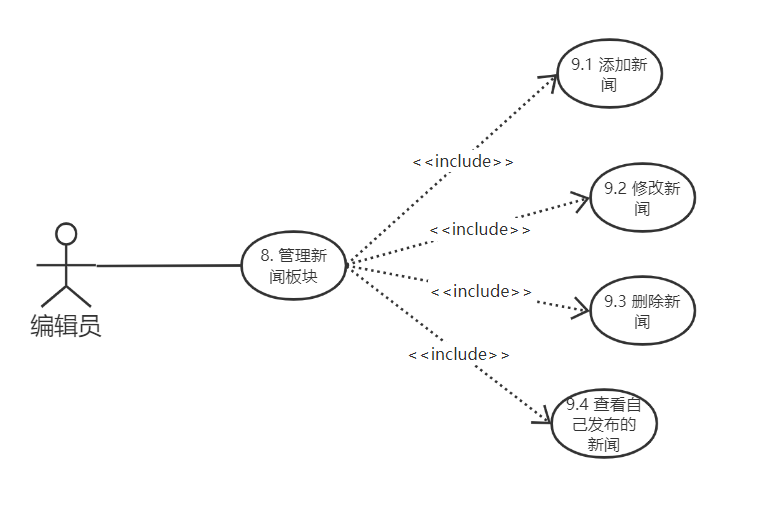
\includegraphics[width=.8\textwidth]{ch5/editorUseCase.png}
    \caption{编辑员用例图}\label{fig:editorUseCase}
    \vspace{\baselineskip} % 表示图与正文空一行
\end{figure}

% 16 添加新闻
\begin{table}[htbp]
    \centering
    \caption{添加新闻}
    \vspace{0.5em}\wuhao
    \begin{tabular}{|l|l|l|l|}
        \hline
        \makebox[0.12\textwidth][l]{编号} & \makebox[0.25\textwidth][c]{UC-03 9-1}                  & \makebox[0.15\textwidth][l]{名称} & \makebox[0.3\textwidth][c]{添加新闻}                                          \\
        \hline
        执行者                            & \makebox[0.25\textwidth][c]{编辑员}                     & 优先级                            & \makebox[0.3\textwidth][c]{高 ~$\square$ ~中 ~$\blacksquare$~ 低 ~$\square$~} \\
        \hline
        描述                              & \multicolumn{3}{l|}{编辑员即使发布战时新闻并做好分类。}                                                                                                                     \\
        \hline
        前置条件                          & \multicolumn{3}{l|}{无}                                                                                                                                                     \\
        \hline
        基本流程                          & \multicolumn{3}{l|}{
            \begin{minipage}[t]{0.8\textwidth}
                \begin{enumerate}
                    \item 点击添加新闻按钮。
                    \item 填写基本信息,并提交
                \end{enumerate}
                \vspace{.5em}
            \end{minipage}
        }                                                                                                                                                                                                               \\
        \hline
        结束状况                          & \multicolumn{3}{l|}{数据库增加新闻数据。    }                                                                                                                               \\
        \hline
        可选流程                          & \multicolumn{3}{l|}{点击取消按钮取消新闻的编辑发布。 }                                                                                                                      \\
        \hline
        异常流程                          & \multicolumn{3}{l|}{无}                                                                                                                                                     \\
        \hline
        说明                              & \multicolumn{3}{l|}{无}                                                                                                                                                     \\
        \hline
    \end{tabular}
\end{table}

% 17 修改新闻
\begin{table}[htbp]
    \centering
    \caption{修改新闻}
    \vspace{0.5em}\wuhao
    \begin{tabular}{|l|l|l|l|}
        \hline
        \makebox[0.12\textwidth][l]{编号} & \makebox[0.25\textwidth][c]{UC-03 9-2}               & \makebox[0.15\textwidth][l]{名称} & \makebox[0.3\textwidth][c]{修改新闻内容}                                      \\
        \hline
        执行者                            & \makebox[0.25\textwidth][c]{编辑员}                  & 优先级                            & \makebox[0.3\textwidth][c]{高 ~$\square$ ~中 ~$\blacksquare$~ 低 ~$\square$~} \\
        \hline
        描述                              & \multicolumn{3}{l|}{
        \begin{minipage}[t]{0.8\textwidth}
                新闻被举报并且审核通过之后或者编辑员想要自己修改,会下架新闻并通知编辑员修改新闻再次发布。
            \end{minipage}}                                                                                                                                                                                  \\
        \hline
        前置条件                          & \multicolumn{3}{l|}{无}                                                                                                                                                  \\
        \hline
        基本流程                          & \multicolumn{3}{l|}{
            \begin{minipage}[t]{0.8\textwidth}
                \begin{enumerate}
                    \item   查看自己发布的新闻列表。
                    \item 进入具体的新闻编辑管理页面,修改并发布。
                \end{enumerate}
                \vspace{.5em}
            \end{minipage}
        }                                                                                                                                                                                                            \\
        \hline
        结束状况                          & \multicolumn{3}{l|}{数据库修改新闻数据。    }                                                                                                                            \\
        \hline
        可选流程                          & \multicolumn{3}{l|}{点击取消按钮取消对新闻的修改。 }                                                                                                                     \\
        \hline
        异常流程                          & \multicolumn{3}{l|}{无}                                                                                                                                                  \\
        \hline
        说明                              & \multicolumn{3}{l|}{无}                                                                                                                                                  \\
        \hline
    \end{tabular}
\end{table}

% 18 删除新闻
\begin{table}[htbp]
    \centering
    \caption{删除新闻}
    \vspace{0.5em}\wuhao
    \begin{tabular}{|l|l|l|l|}
        \hline
        \makebox[0.12\textwidth][l]{编号} & \makebox[0.25\textwidth][c]{UC-03 9-3}                              & \makebox[0.15\textwidth][l]{名称} & \makebox[0.3\textwidth][c]{删除新闻信息}                                      \\
        \hline
        执行者                            & \makebox[0.25\textwidth][c]{编辑员}                                 & 优先级                            & \makebox[0.3\textwidth][c]{高 ~$\blacksquare$ ~中 ~$\square$~ 低 ~$\square$~} \\
        \hline
        描述                              & \multicolumn{3}{l|}{新闻被举报之后管理员会删除新闻并且通知管理员。}                                                                                                                     \\
        \hline
        前置条件                          & \multicolumn{3}{l|}{  编辑员发布了新闻信息。}                                                                                                                                           \\
        \hline
        基本流程                          & \multicolumn{3}{l|}{
            \begin{minipage}[t]{0.8\textwidth}
                \begin{enumerate}
                    \item   查看自己的新闻列表。
                    \item   进入具体的新闻编辑管理页面,进行删除。
                \end{enumerate}
                \vspace{.5em}
            \end{minipage}
        }                                                                                                                                                                                                                           \\
        \hline
        结束状况                          & \multicolumn{3}{l|}{数据库删除新闻信息数据。    }                                                                                                                                       \\
        \hline
        可选流程                          & \multicolumn{3}{l|}{取消删除。}                                                                                                                                                         \\
        \hline
        异常流程                          & \multicolumn{3}{l|}{无}                                                                                                                                                                 \\
        \hline
        说明                              & \multicolumn{3}{l|}{无}                                                                                                                                                                 \\
        \hline
    \end{tabular}
\end{table}

% 19 查看发布新闻
\begin{table}[htbp]
    \centering
    \caption{查看发布新闻}
    \vspace{0.5em}\wuhao
    \begin{tabular}{|l|l|l|l|}
        \hline
        \makebox[0.12\textwidth][l]{编号} & \makebox[0.25\textwidth][c]{UC-03 9-4}               & \makebox[0.15\textwidth][l]{名称} & \makebox[0.3\textwidth][c]{查看新闻信息}                                      \\
        \hline
        执行者                            & \makebox[0.25\textwidth][c]{编辑员}                  & 优先级                            & \makebox[0.3\textwidth][c]{高 ~$\blacksquare$ ~中 ~$\square$~ 低 ~$\square$~} \\
        \hline
        描述                              & \multicolumn{3}{l|}{
        \begin{minipage}[t]{0.8\textwidth}
                目标:


                可以方便的查看自己的房源发布情况,在此基础上做下一步工作。
                \begin{enumerate}
                    \item 查看发布的房源历史信息。
                    \item 点击查看具体房源信息。
                \end{enumerate}
                \vspace{.5em}
            \end{minipage}}                                                                                                                                                                                  \\
        \hline
        前置条件                          & \multicolumn{3}{l|}{房主发布了房源信息。}                                                                                                                                \\
        \hline
        基本流程                          & \multicolumn{3}{l|}{无}                                                                                                                                                  \\
        \hline
        结束状况                          & \multicolumn{3}{l|}{系统的数据不会发生任何变化。   }                                                                                                                     \\
        \hline
        可选流程                          & \multicolumn{3}{l|}{无}                                                                                                                                                  \\
        \hline
        异常流程                          & \multicolumn{3}{l|}{无}                                                                                                                                                  \\
        \hline
        说明                              & \multicolumn{3}{l|}{ 无}                                                                                                                                                 \\
        \hline
    \end{tabular}
\end{table}

\section{管理员用例图}

管理员的用例图如图~\ref{fig:adminUseCase}~所示。

\begin{figure}[htbp]
    \centering
    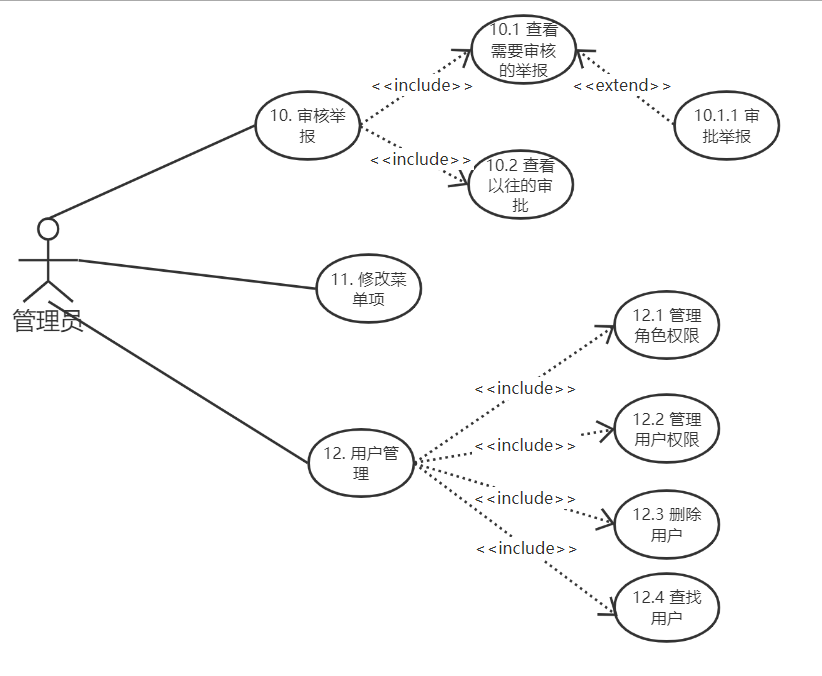
\includegraphics[width=.8\textwidth]{ch5/adminUseCase.png}
    \caption{管理员用例图}\label{fig:adminUseCase}
    \vspace{\baselineskip} % 表示图与正文空一行
\end{figure}

% 20 查看待审核举报
\begin{table}[htbp]
    \centering
    \caption{查看待审核举报}
    \vspace{0.5em}\wuhao
    \begin{tabular}{|l|l|l|l|}
        \hline
        \makebox[0.12\textwidth][l]{编号} & \makebox[0.25\textwidth][c]{UC-04 10-1 }             & \makebox[0.15\textwidth][l]{名称} & \makebox[0.3\textwidth][c]{查看待审核举报}                                    \\
        \hline
        执行者                            & \makebox[0.25\textwidth][c]{管理员}                  & 优先级                            & \makebox[0.3\textwidth][c]{高 ~$\blacksquare$ ~中 ~$\square$~ 低 ~$\square$~} \\
        \hline
        描述                              & \multicolumn{3}{l|}{
        \begin{minipage}[t]{0.8\textwidth}
                目标:

                部门经历需要方便的查看需要审核的申请,并在此基础上可以方便的审核。

                具体要求:
                \begin{enumerate}
                    \item 系统按照默认按照申请提出时间的顺序,列出状态为“待定”的举报申请列表。
                    \item 系统需要能够显示举报的基本信息。
                    \item 用户可以直接在举报列表界面审核通过,也可以在具体的举报界面审核。
                \end{enumerate}
                \vspace{.5em}
            \end{minipage}}                                                                                                                                                                                  \\
        \hline
        前置条件                          & \multicolumn{3}{l|}{有需要审核的举报。}                                                                                                                                  \\
        \hline
        结束状况                          & \multicolumn{3}{l|}{系统的数据不会发生任何变化。   }                                                                                                                     \\
        \hline
        可选流程                          & \multicolumn{3}{l|}{无}                                                                                                                                                  \\
        \hline
        说明                              & \multicolumn{3}{l|}{
            \begin{minipage}[t]{0.8\textwidth}
                \begin{enumerate}
                    \item 需要管理员审核的是状态为“待定”的申请。
                    \item 申请者提出举报申请之后,申请状态为“待定”。
                    \item 申请者修改被拒绝的举报之后,申请状态为“待定”。
                \end{enumerate}
                \vspace{.5em}
            \end{minipage}
        }                                                                                                                                                                                                            \\
        \hline
    \end{tabular}
\end{table}

% 21 审核举报
\begin{table}[htbp]
    \centering
    \caption{审核举报}
    \vspace{0.5em}\wuhao
    \begin{tabular}{|l|l|l|l|}
        \hline
        \makebox[0.12\textwidth][l]{编号} & \makebox[0.25\textwidth][c]{UC-04 10-1-1 }                                & \makebox[0.15\textwidth][l]{名称} & \makebox[0.3\textwidth][c]{审核举报}                                          \\
        \hline
        执行者                            & \makebox[0.25\textwidth][c]{管理员}                                       & 优先级                            & \makebox[0.3\textwidth][c]{高 ~$\blacksquare$ ~中 ~$\square$~ 低 ~$\square$~} \\
        \hline
        描述                              & \multicolumn{3}{l|}{
        \begin{minipage}[t]{0.8\textwidth}
                目标:

                用户能根据举报申请,审核该举报。

                具体要求:
                \begin{enumerate}
                    \item 用户可以直接在举报列表界面审核通过,也可以在具体的举报界面审核。
                    \item 审核的时候需要选择批准或拒绝,同时输入审核理由。
                    \item 审核时间不需要用户填入,由系统自动填入。
                \end{enumerate}
                \vspace{.5em}
            \end{minipage}}                                                                                                                                                                                                       \\
        \hline
        前置条件                          & \multicolumn{3}{l|}{有需要审核的举报。}                                                                                                                                                       \\
        \hline
        结束状况                          & \multicolumn{3}{l|}{系统根据用户的审核结果来更改数据库中对应消息的状态。}                                                                                                                     \\
        \hline
        可选流程                          & \multicolumn{3}{l|}{无}                                                                                                                                                                       \\
        \hline
        说明                              & \multicolumn{3}{l|}{无}                                                                                                                                                                       \\
        \hline
    \end{tabular}
\end{table}

% 22 查看以往的审核
\begin{table}[htbp]
    \centering
    \caption{查看以往的审核}
    \vspace{0.5em}\wuhao
    \begin{tabular}{|l|l|l|l|}
        \hline
        \makebox[0.12\textwidth][l]{编号} & \makebox[0.25\textwidth][c]{UC-04 10-2 }          & \makebox[0.15\textwidth][l]{名称} & \makebox[0.3\textwidth][c]{查看审核}                                          \\
        \hline
        执行者                            & \makebox[0.25\textwidth][c]{管理员}               & 优先级                            & \makebox[0.3\textwidth][c]{高 ~$\square$ ~中 ~$\blacksquare$~ 低 ~$\square$~} \\
        \hline
        描述                              & \multicolumn{3}{l|}{
        \begin{minipage}[t]{0.8\textwidth}
                目标:

                用户能够方便的查看曾经审批过的举报。

                具体要求:
                \begin{enumerate}
                    \item 系统按照默认按照申请提出时间的顺序,列出状态为“待定”的举报申请列表。
                    \item 系统需要能够显示举报的基本信息和状态。
                \end{enumerate}
                \vspace{.5em}
            \end{minipage}}                                                                                                                                                                               \\
        \hline
        前置条件                          & \multicolumn{3}{l|}{无}                                                                                                                                               \\
        \hline
        结束状况                          & \multicolumn{3}{l|}{系统的数据不会发生任何变化。}                                                                                                                     \\
        \hline
        可选流程                          & \multicolumn{3}{l|}{无}                                                                                                                                               \\
        \hline
        说明                              & \multicolumn{3}{l|}{无}                                                                                                                                               \\
        \hline
    \end{tabular}
\end{table}

% 23 修改菜单项
\begin{table}[htbp]
    \centering
    \caption{修改菜单项}
    \vspace{0.5em}\wuhao
    \begin{tabular}{|l|l|l|l|}
        \hline
        \makebox[0.12\textwidth][l]{编号} & \makebox[0.25\textwidth][c]{UC-04 11 }            & \makebox[0.15\textwidth][l]{名称} & \makebox[0.3\textwidth][c]{修改菜单项}                                        \\
        \hline
        执行者                            & \makebox[0.25\textwidth][c]{管理员}               & 优先级                            & \makebox[0.3\textwidth][c]{高 ~$\blacksquare$ ~中 ~$\square$~ 低 ~$\square$~} \\
        \hline
        描述                              & \multicolumn{3}{l|}{
        \begin{minipage}[t]{0.8\textwidth}
                目标:

                管理员能更改用户角色的菜单项

                具体要求:
                \begin{enumerate}
                    \item 管理员需要能够更改用户的下来菜单项。
                \end{enumerate}
                \vspace{.5em}
            \end{minipage}}                                                                                                                                                                               \\
        \hline
        前置条件                          & \multicolumn{3}{l|}{无}                                                                                                                                               \\
        \hline
        结束状况                          & \multicolumn{3}{l|}{系统的数据不会发生任何变化。}                                                                                                                     \\
        \hline
        说明                              & \multicolumn{3}{l|}{无}                                                                                                                                               \\
        \hline
    \end{tabular}
\end{table}

% 24 管理角色权限
\begin{table}[htbp]
    \centering
    \caption{管理角色权限}
    \vspace{0.5em}\wuhao
    \begin{tabular}{|l|l|l|l|}
        \hline
        \makebox[0.12\textwidth][l]{编号} & \makebox[0.25\textwidth][c]{UC-04 12.1 }                            & \makebox[0.15\textwidth][l]{名称} & \makebox[0.3\textwidth][c]{管理角色权限}                                      \\
        \hline
        执行者                            & \makebox[0.25\textwidth][c]{管理员}                                 & 优先级                            & \makebox[0.3\textwidth][c]{高 ~$\blacksquare$ ~中 ~$\square$~ 低 ~$\square$~} \\
        \hline
        描述                              & \multicolumn{3}{l|}{
        \begin{minipage}[t]{0.8\textwidth}
                目标:

                管理员能更改具体角色的权限
                \vspace{.5em}
            \end{minipage}}                                                                                                                                                                                                 \\
        \hline
        前置条件                          & \multicolumn{3}{l|}{无}                                                                                                                                                                 \\
        \hline
        基本流程                          & \multicolumn{3}{l|}{无}                                                                                                                                                                 \\
        \hline
        结束状况                          & \multicolumn{3}{l|}{用户角色权限发生变化。}                                                                                                                                             \\
        \hline
        异常流程                          & \multicolumn{3}{l|}{无}                                                                                                                                                                 \\
        \hline
        说明                              & \multicolumn{3}{l|}{管理员能够对于某一角色的用户的权限做集体更改。}                                                                                                                     \\
        \hline
    \end{tabular}
\end{table}

% 25 管理用户权限
\begin{table}[htbp]
    \centering
    \caption{管理用户权限}
    \vspace{0.5em}\wuhao
    \begin{tabular}{|l|l|l|l|}
        \hline
        \makebox[0.12\textwidth][l]{编号} & \makebox[0.25\textwidth][c]{UC-04 12-2 }                                      & \makebox[0.15\textwidth][l]{名称} & \makebox[0.3\textwidth][c]{管理用户权限}                                      \\
        \hline
        执行者                            & \makebox[0.25\textwidth][c]{管理员}                                           & 优先级                            & \makebox[0.3\textwidth][c]{高 ~$\blacksquare$ ~中 ~$\square$~ 低 ~$\square$~} \\
        \hline
        描述                              & \multicolumn{3}{l|}{
        \begin{minipage}[t]{0.8\textwidth}
                目标:

                管理员能更改具体某一用户的权限
                \vspace{.5em}
            \end{minipage}}                                                                                                                                                                                                           \\
        \hline
        前置条件                          & \multicolumn{3}{l|}{无}                                                                                                                                                                           \\
        \hline
        结束状况                          & \multicolumn{3}{l|}{用户权限发生变化。}                                                                                                                                                           \\
        \hline
        说明                              & \multicolumn{3}{l|}{管理员能够对于具体的用户的某些操作的权限进行剥夺和赋予。}                                                                                                                     \\
        \hline
    \end{tabular}
\end{table}

% 26 删除用户
\begin{table}[htbp]
    \centering
    \caption{删除用户}
    \vspace{0.5em}\wuhao
    \begin{tabular}{|l|l|l|l|}
        \hline
        \makebox[0.12\textwidth][l]{编号} & \makebox[0.25\textwidth][c]{UC-04 12-3 }                  & \makebox[0.15\textwidth][l]{名称} & \makebox[0.3\textwidth][c]{删除用户}                                          \\
        \hline
        执行者                            & \makebox[0.25\textwidth][c]{管理员}                       & 优先级                            & \makebox[0.3\textwidth][c]{高 ~$\blacksquare$ ~中 ~$\square$~ 低 ~$\square$~} \\
        \hline
        描述                              & \multicolumn{3}{l|}{管理员可以删除用户,禁止用户再次登录}                                                                                                                     \\
        \hline
        前置条件                          & \multicolumn{3}{l|}{无}                                                                                                                                                       \\
        \hline
        基本流程                          & \multicolumn{3}{l|}{无}                                                                                                                                                       \\
        \hline
        结束状况                          & \multicolumn{3}{l|}{修改用户在数据库中的状态。}                                                                                                                               \\
        \hline
        异常流程                          & \multicolumn{3}{l|}{无}                                                                                                                                                       \\
        \hline
        说明                              & \multicolumn{3}{l|}{
        \begin{minipage}[t]{0.8\textwidth}
                管理员对于用户的增删改查,增加的是编辑员账号信息;删除不合规的账号用户;对于用户的修改包括权限等在用例图UC-04 12-1 和12-2做了介绍.
                \vspace{.5em}
            \end{minipage}}                                                                                                                                                                                       \\
        \hline
    \end{tabular}
\end{table}

% 27 查找用户
\begin{table}[htbp]
    \centering
    \caption{删除用户}
    \vspace{0.5em}\wuhao
    \begin{tabular}{|l|l|l|l|}
        \hline
        \makebox[0.12\textwidth][l]{编号} & \makebox[0.25\textwidth][c]{UC-04 12-4 }                        & \makebox[0.15\textwidth][l]{名称} & \makebox[0.3\textwidth][c]{查找用户}                                          \\
        \hline
        执行者                            & \makebox[0.25\textwidth][c]{管理员}                             & 优先级                            & \makebox[0.3\textwidth][c]{高 ~$\square$ ~中 ~$\blacksquare$~ 低 ~$\square$~} \\
        \hline
        描述                              & \multicolumn{3}{l|}{管理员查找指定用户,在此基础上做继续操作。}                                                                                                                     \\
        \hline
        前置条件                          & \multicolumn{3}{l|}{无}                                                                                                                                                             \\
        \hline
        基本流程                          & \multicolumn{3}{l|}{无}                                                                                                                                                             \\
        \hline
        结束状况                          & \multicolumn{3}{l|}{修改用户在数据库中的状态。}                                                                                                                                     \\
        \hline
        异常流程                          & \multicolumn{3}{l|}{无}                                                                                                                                                             \\
        \hline
        说明                              & \multicolumn{3}{l|}{
        \begin{minipage}[t]{0.8\textwidth}
                查找用户,在在此基础上对用户的权限进行操作。
            \end{minipage}}                                                                                                                                                                                             \\
        \hline
    \end{tabular}
\end{table}
\chapter{非功能性需求}
\section{系统架构要求}
系统的构件图如图~\ref{fig:goujian}~所示。
\begin{figure}[htbp]
    \centering
    \includegraphics[width=\textwidth]{ch6/goujian.png}
    \caption{系统构件图}\label{fig:goujian}
    \vspace{\baselineskip} % 表示图与正文空一行
\end{figure}
系统的架构图如图~\ref{fig:jiagou}~所示。
\begin{figure}[htbp]
    \centering
    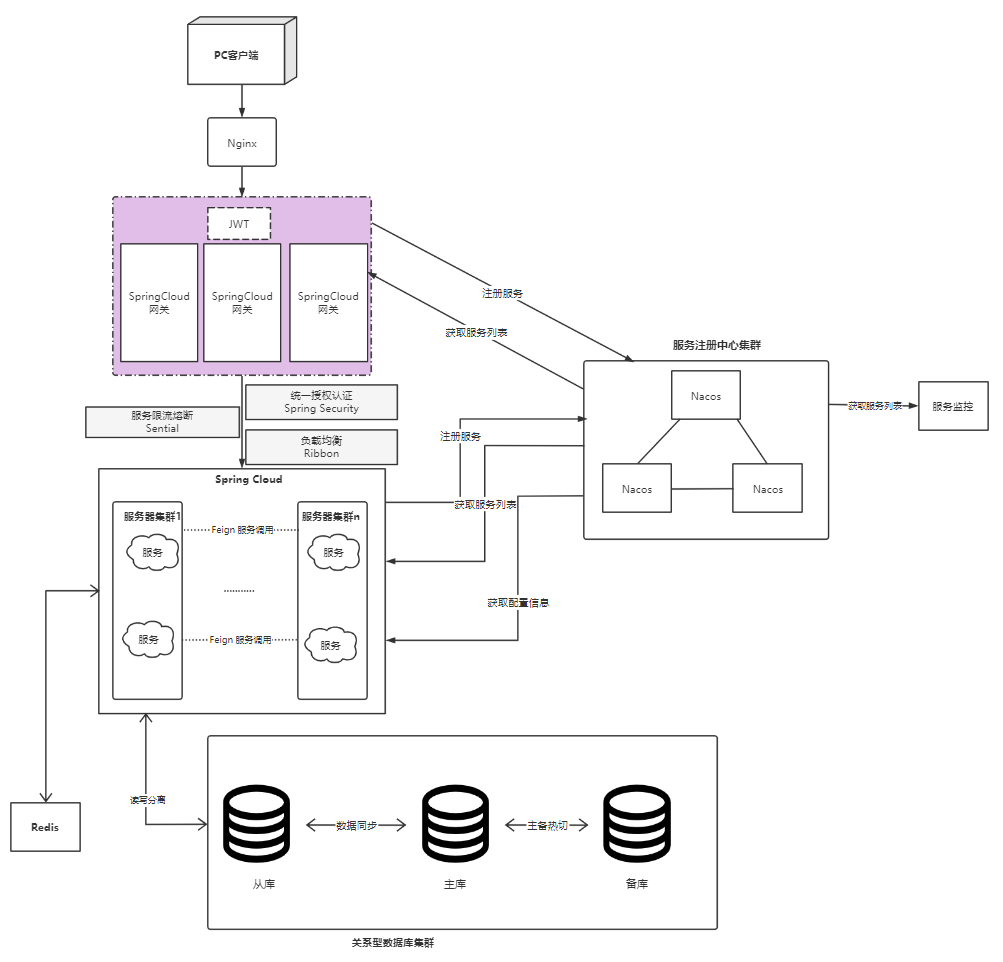
\includegraphics[width=\textwidth]{ch6/bushu.png}
    \caption{系统部署图}\label{fig:jiagou}
    \vspace{\baselineskip} % 表示图与正文空一行
\end{figure}
\section{接口}
\textbf{待填写}
\section{安全性}
\begin{enumerate}
    \item 房主发布房源必须要进行身份认证,已保障难民的安全。对于房主的身份信息保证保密。
    \item 可以做到维持,不过用户更换客户机的时候需要重新登录(已认证则不必再次认证)。
    \item 难民有举报功能,要是需要使用此功能,需要登录。
    \item 设计过程需要充分的考虑到恶意代码的非法入侵行为,保证达到安全可靠性最高。
\end{enumerate}
\section{性能}
\subsection{时间需求}
\begin{enumerate}
    \item 查询时间的最长等待时间不超过2秒
    \item 更新信息的最长时间不超过3秒
    \item 数据上传和下载时间最长不超过3秒
\end{enumerate}
\subsection{空间需求}
\begin{enumerate}
    \item 支持的终端数不超过10000
    \item 支持并行操作的使用者不超过5000
    \item 记录处理数:10000
\end{enumerate}
\section{设计约束}
\begin{enumerate}
    \item 建议硬盘:128GB 或更高
    \item 建议内存:256MB 或更高
    \item 建议CPU:1.4GHZ 或更高
    \item 网络环境:广域网/局域网。有线网络访问速度更快。
\end{enumerate}
\section{界面}
\textbf{待填写}
\chapter{附录}
\chapter{版本修订记录}
\begin{table}[htbp]
    \centering
    \caption{涉众分析表}
    \label{tab:xuqiu}
    \vspace{0.5em}\wuhao
    \begin{tabular}{|c|c|c|c|}
        \hline
\makebox[0.2\textwidth][c]{日期} & \makebox[0.2\textwidth][c]{作者} & \makebox[0.4\textwidth][c]{内容提要} & \makebox[0.1\textwidth][c]{版本} \\
        \hline
        2022/3/29                        & \makecell[c]{俞林昊 \quad 李浠贤                                                                           \\ 左江涛 \quad 杜义恒} & 定出需求框架                         & 0.1                              \\
        \hline
2022/4/5                         & 俞林昊                           & \begin{minipage}[t]{.4\textwidth}
    包含活动图,状态图,时序图,用例图的业务流程分析和功能性需求/非功能性需求。
    \vspace{.5em}
\end{minipage}            & 0.2                              \\
\hline
2022/4/8                         & 杜义恒                           &
\begin{minipage}[t]{.4\textwidth}
    完成了包含对应需求的类图设计的业务概念分析板块。
    \vspace{.5em}
\end{minipage}        & 0.3                                                                                                        \\
        \hline
    \end{tabular}
\end{table}

	% \clearpage

\end{CJK*}                                     % 结束中文字体使用
\end{document}                                 % 结束全文
